\label{chap:results}

This chapter reports the Phase~1 results in the order of the research questions. Every number comes from a saved result file of the project (Appendix~\ref{app:repro}).

\section{BSISO Season}
\label{sec:res-season}

The BSISO index reproduced from the project's own OLR and u850 anomalies has leading modes explaining 11.2\% and 7.7\% of the variance, close to the approximately 10\% and 7\% reported by Lee \emph{et al.}~\cite{lee2013realtime}. The slightly larger values are consistent with the smaller domain, whose northern edge is 30\dg N rather than 40\dg N. The activity-based season (Figure~\ref{fig:season}) lasts 208 days per year on average, ranges from 82 to 286 days, and begins between April and July. A fixed May--October window would therefore include inactive weeks in some years and miss active weeks in others.

\begin{figure}[htbp]
\centering
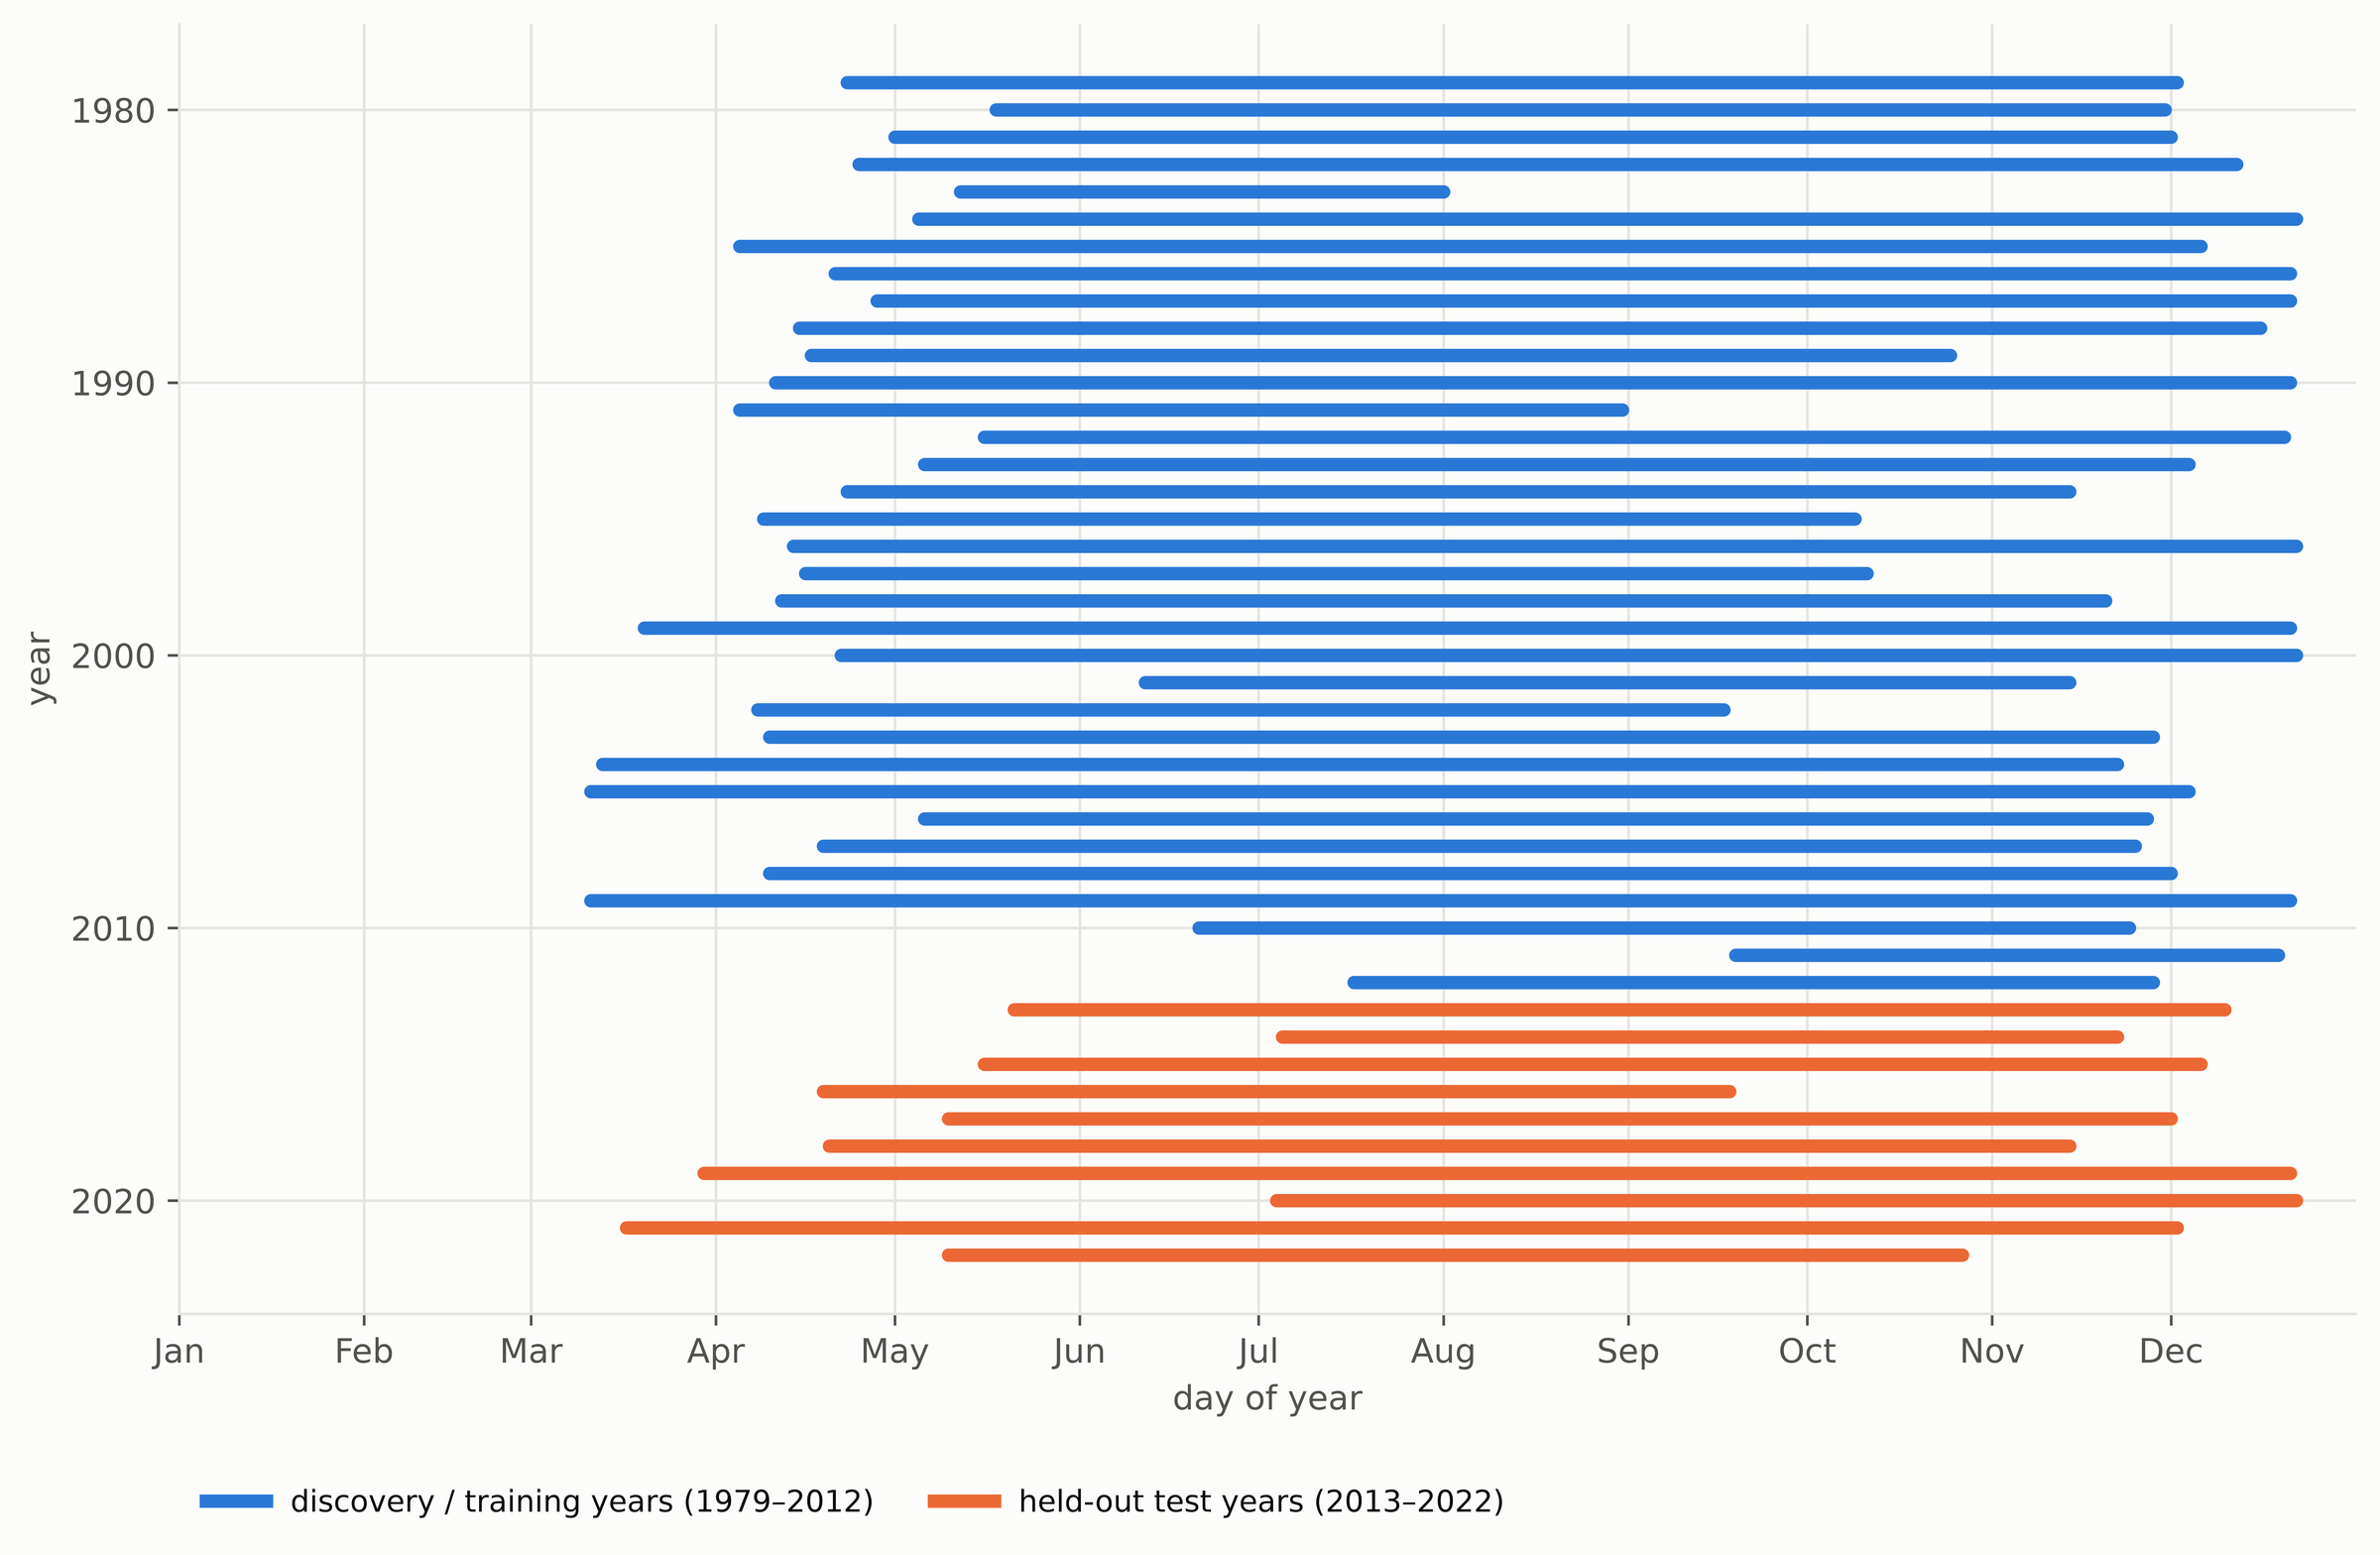
\includegraphics[width=0.82\textwidth]{ppt_01b_active_bsiso_season_per_year.png}
\caption{Active BSISO season (target days) in each year, derived from the reproduced BSISO index. Blue: discovery and training years (1979--2012); orange: held-out test years (2013--2022).}
\label{fig:season}
\end{figure}

\section{Stage A: The Discovered Graph (RQ1)}
\label{sec:res-stagea}

PCMCI at an FDR of 0.05 retains \textbf{536 links} into the 50 OLR targets, 10.7 per target, out of 900{,}000 candidates: the graph is very sparse. Of these, 376 lie within the target's own region, mostly its own OLR at lags of 1--7 days, and 160 come from other regions: OLR 72, u850 37, u200 22, h850 18, PW 11 and SST 0. The outside links act quickly, with a median lag of one day, 90\% at two days or less, and none at 25 days or more. Once PCMCI conditions on these fast drivers, slow precursors such as SST carry little \emph{direct} information, because their influence has already passed through the atmospheric fields. Convection in a neighbouring region, together with the low-level flow that carries moisture and the upper-level wave response, precedes convection in the target, which is the expected physical picture of propagating convection.

Figure~\ref{fig:graphmap} maps the outside drivers. Most connect neighbouring regions; a few longer links carried by wind and height fields span thousands of kilometres within one or two days, at equatorial-wave speeds.

\begin{figure}[htbp]
\centering
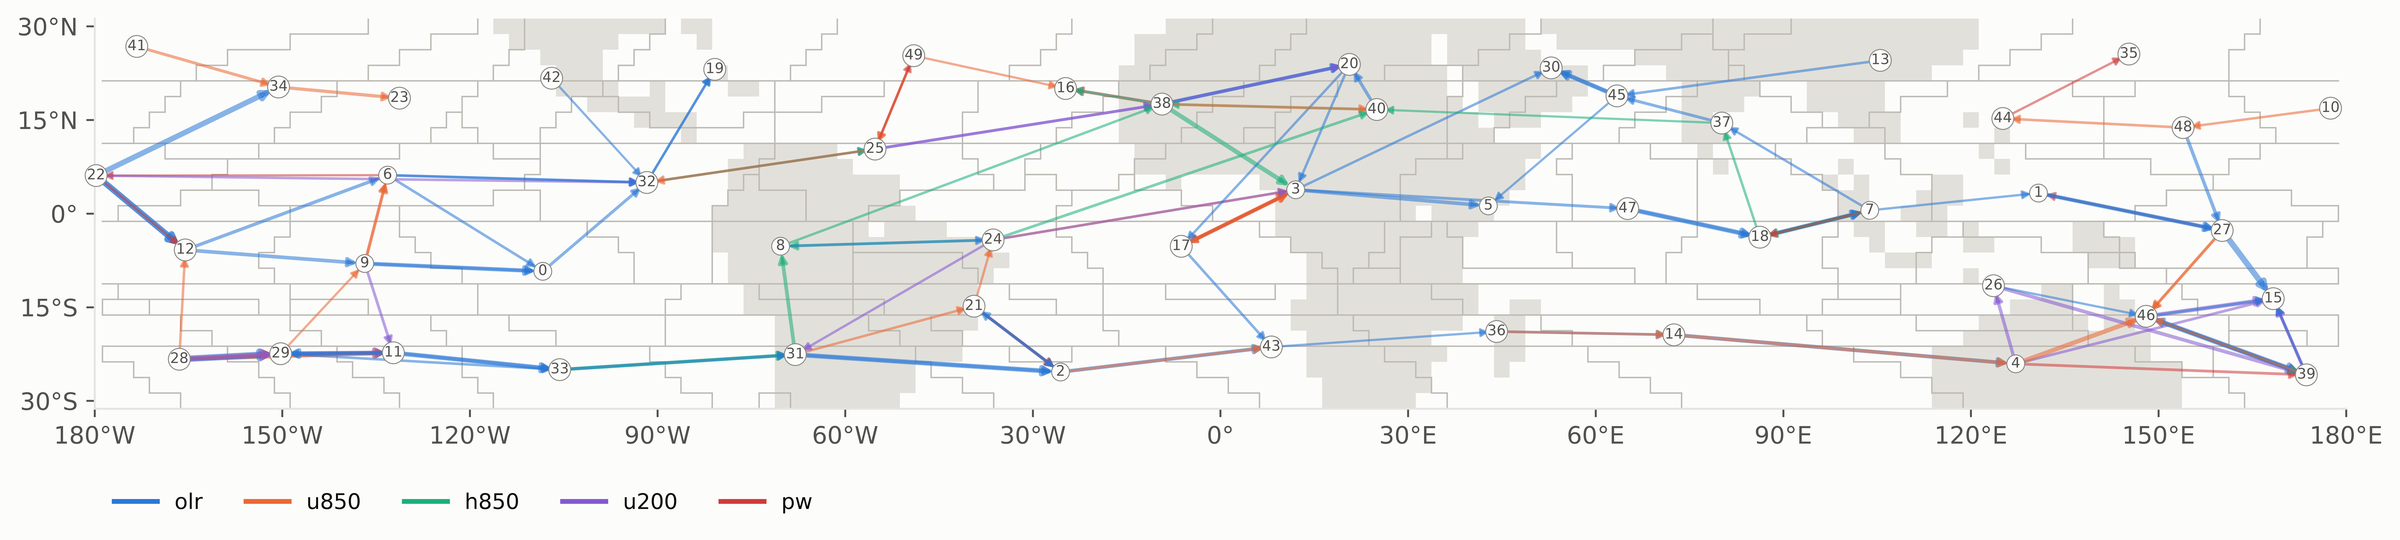
\includegraphics[width=\textwidth]{ppt_map_standard_180_convention.png}
\caption{Validated outside drivers of the 50 OLR targets (arrows from source region to target region), coloured by the source field.}
\label{fig:graphmap}
\end{figure}

\paragraph{Worked example: region 22.} Region 22 lies over the equatorial western Pacific near the Maritime Continent. PCMCI finds 13 links for it: 10 within the region and three from outside (h850 from region 27 at lags 1 and 3, and PW from region 6 at lag 2). Both source regions are about 280\,km away, so the implied speeds of 1--3\ms\ are physically easy. The prior is region 27 (strength 0.21) and region 6 (0.05). Independently, the splitter trained with no prior selects regions 6, 12 and 27, which include both prior regions: two unrelated methods agree on the same drivers. Table~\ref{tab:region22} follows the region's links through the checks.

\begin{table}[htbp]
\centering
\caption{The links of target region 22 through Stages A and B.}
\label{tab:region22}
\footnotesize
\renewcommand{\arraystretch}{1.15}
\begin{tabularx}{\textwidth}{>{\raggedright\arraybackslash}p{2.3cm}>{\centering\arraybackslash}p{1.6cm}>{\raggedright\arraybackslash}X}
\toprule
\textbf{Step} & \textbf{Links} & \textbf{What happened} \\
\midrule
PCMCI & 13 & 10 own-region (OLR lags 1--3, 5--7; u850, h850 lags 1--2); h850 from region 27 (lags 1, 3); PW from region 6 (lag 2) \\
B1 decoys & 13 & no decoy selected anywhere \\
B2 lag mask & 13 & sources $\approx$280\,km away; 1--3\ms \\
B3 top-$k$ & 3 outside & all three outside links kept \\
B4 persistence & 0.67 & both region-27 links persist; region-6 PW link flagged \\
Prior & 2 regions & region 27 (0.21), region 6 (0.05) \\
\bottomrule
\end{tabularx}
\end{table}

\section{Stage B: Validation (RQ2)}
\label{sec:res-stageb}

\begin{figure}[htbp]
\centering
\begin{subfigure}[b]{0.56\textwidth}\centering
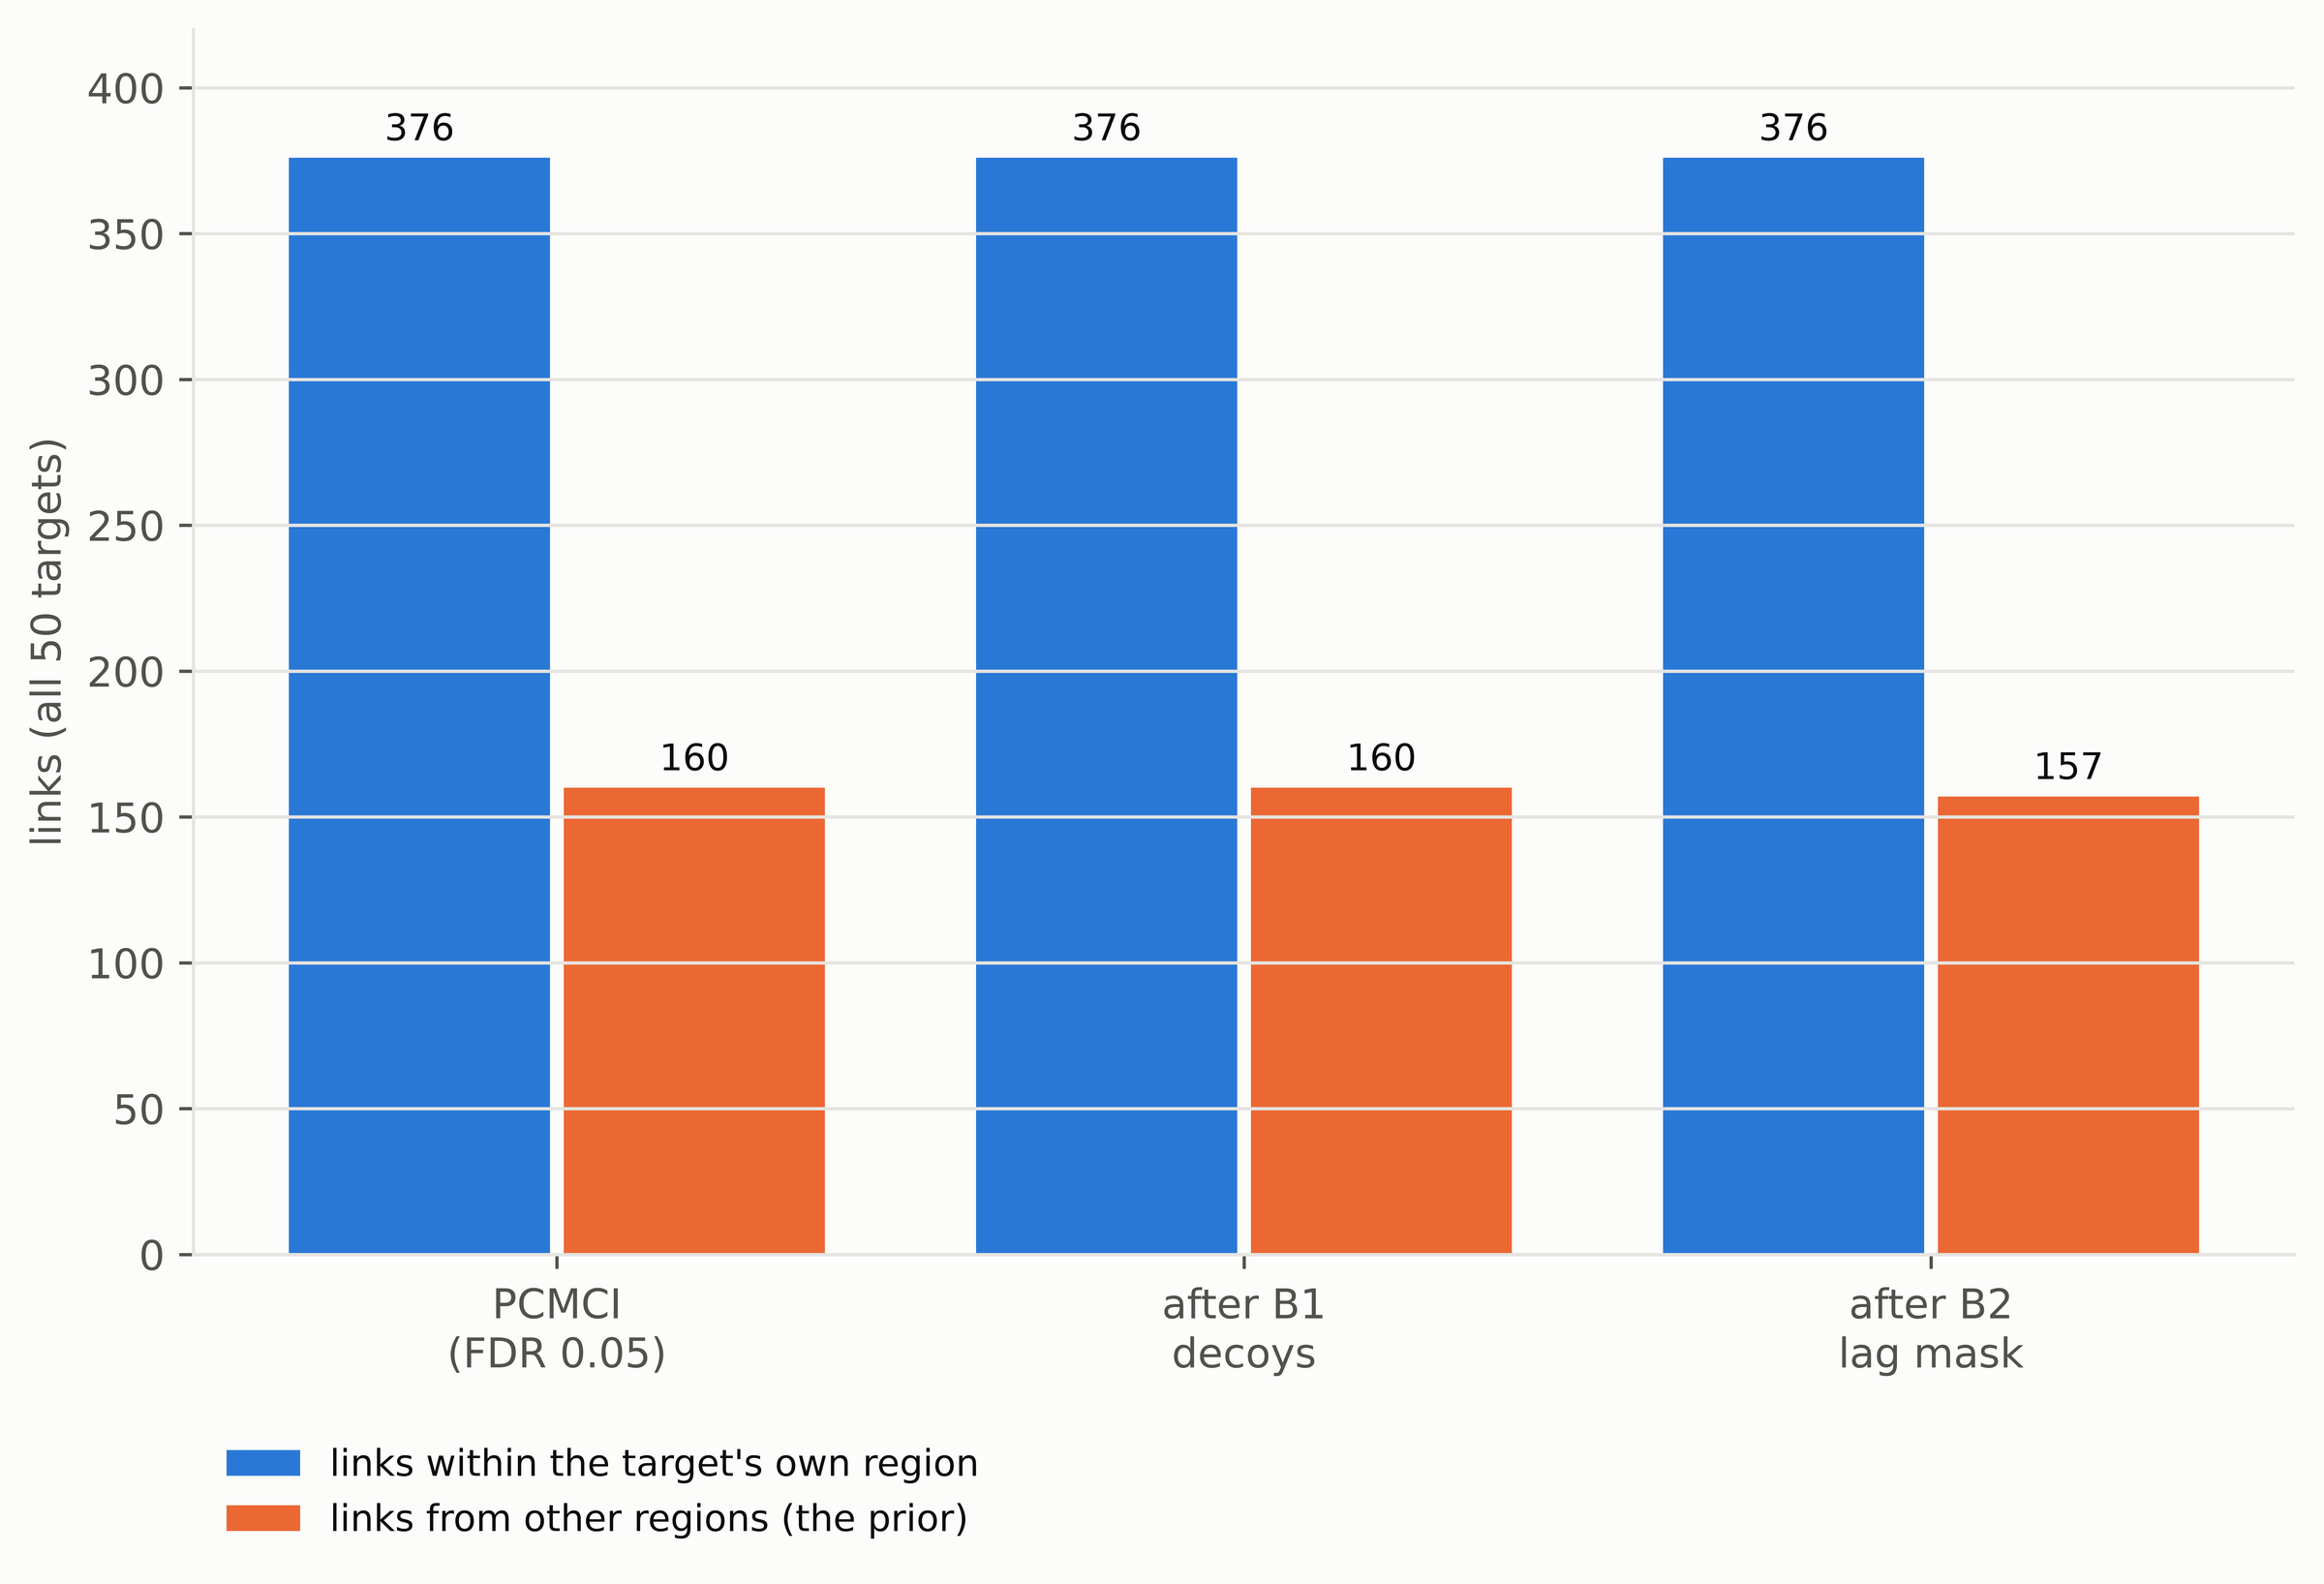
\includegraphics[width=\textwidth]{ppt_03b_links_through_checks_no_b3_b4.png}
\caption{Links after PCMCI, B1 and B2.}\label{fig:links}
\end{subfigure}\hfill
\begin{subfigure}[b]{0.4\textwidth}\centering
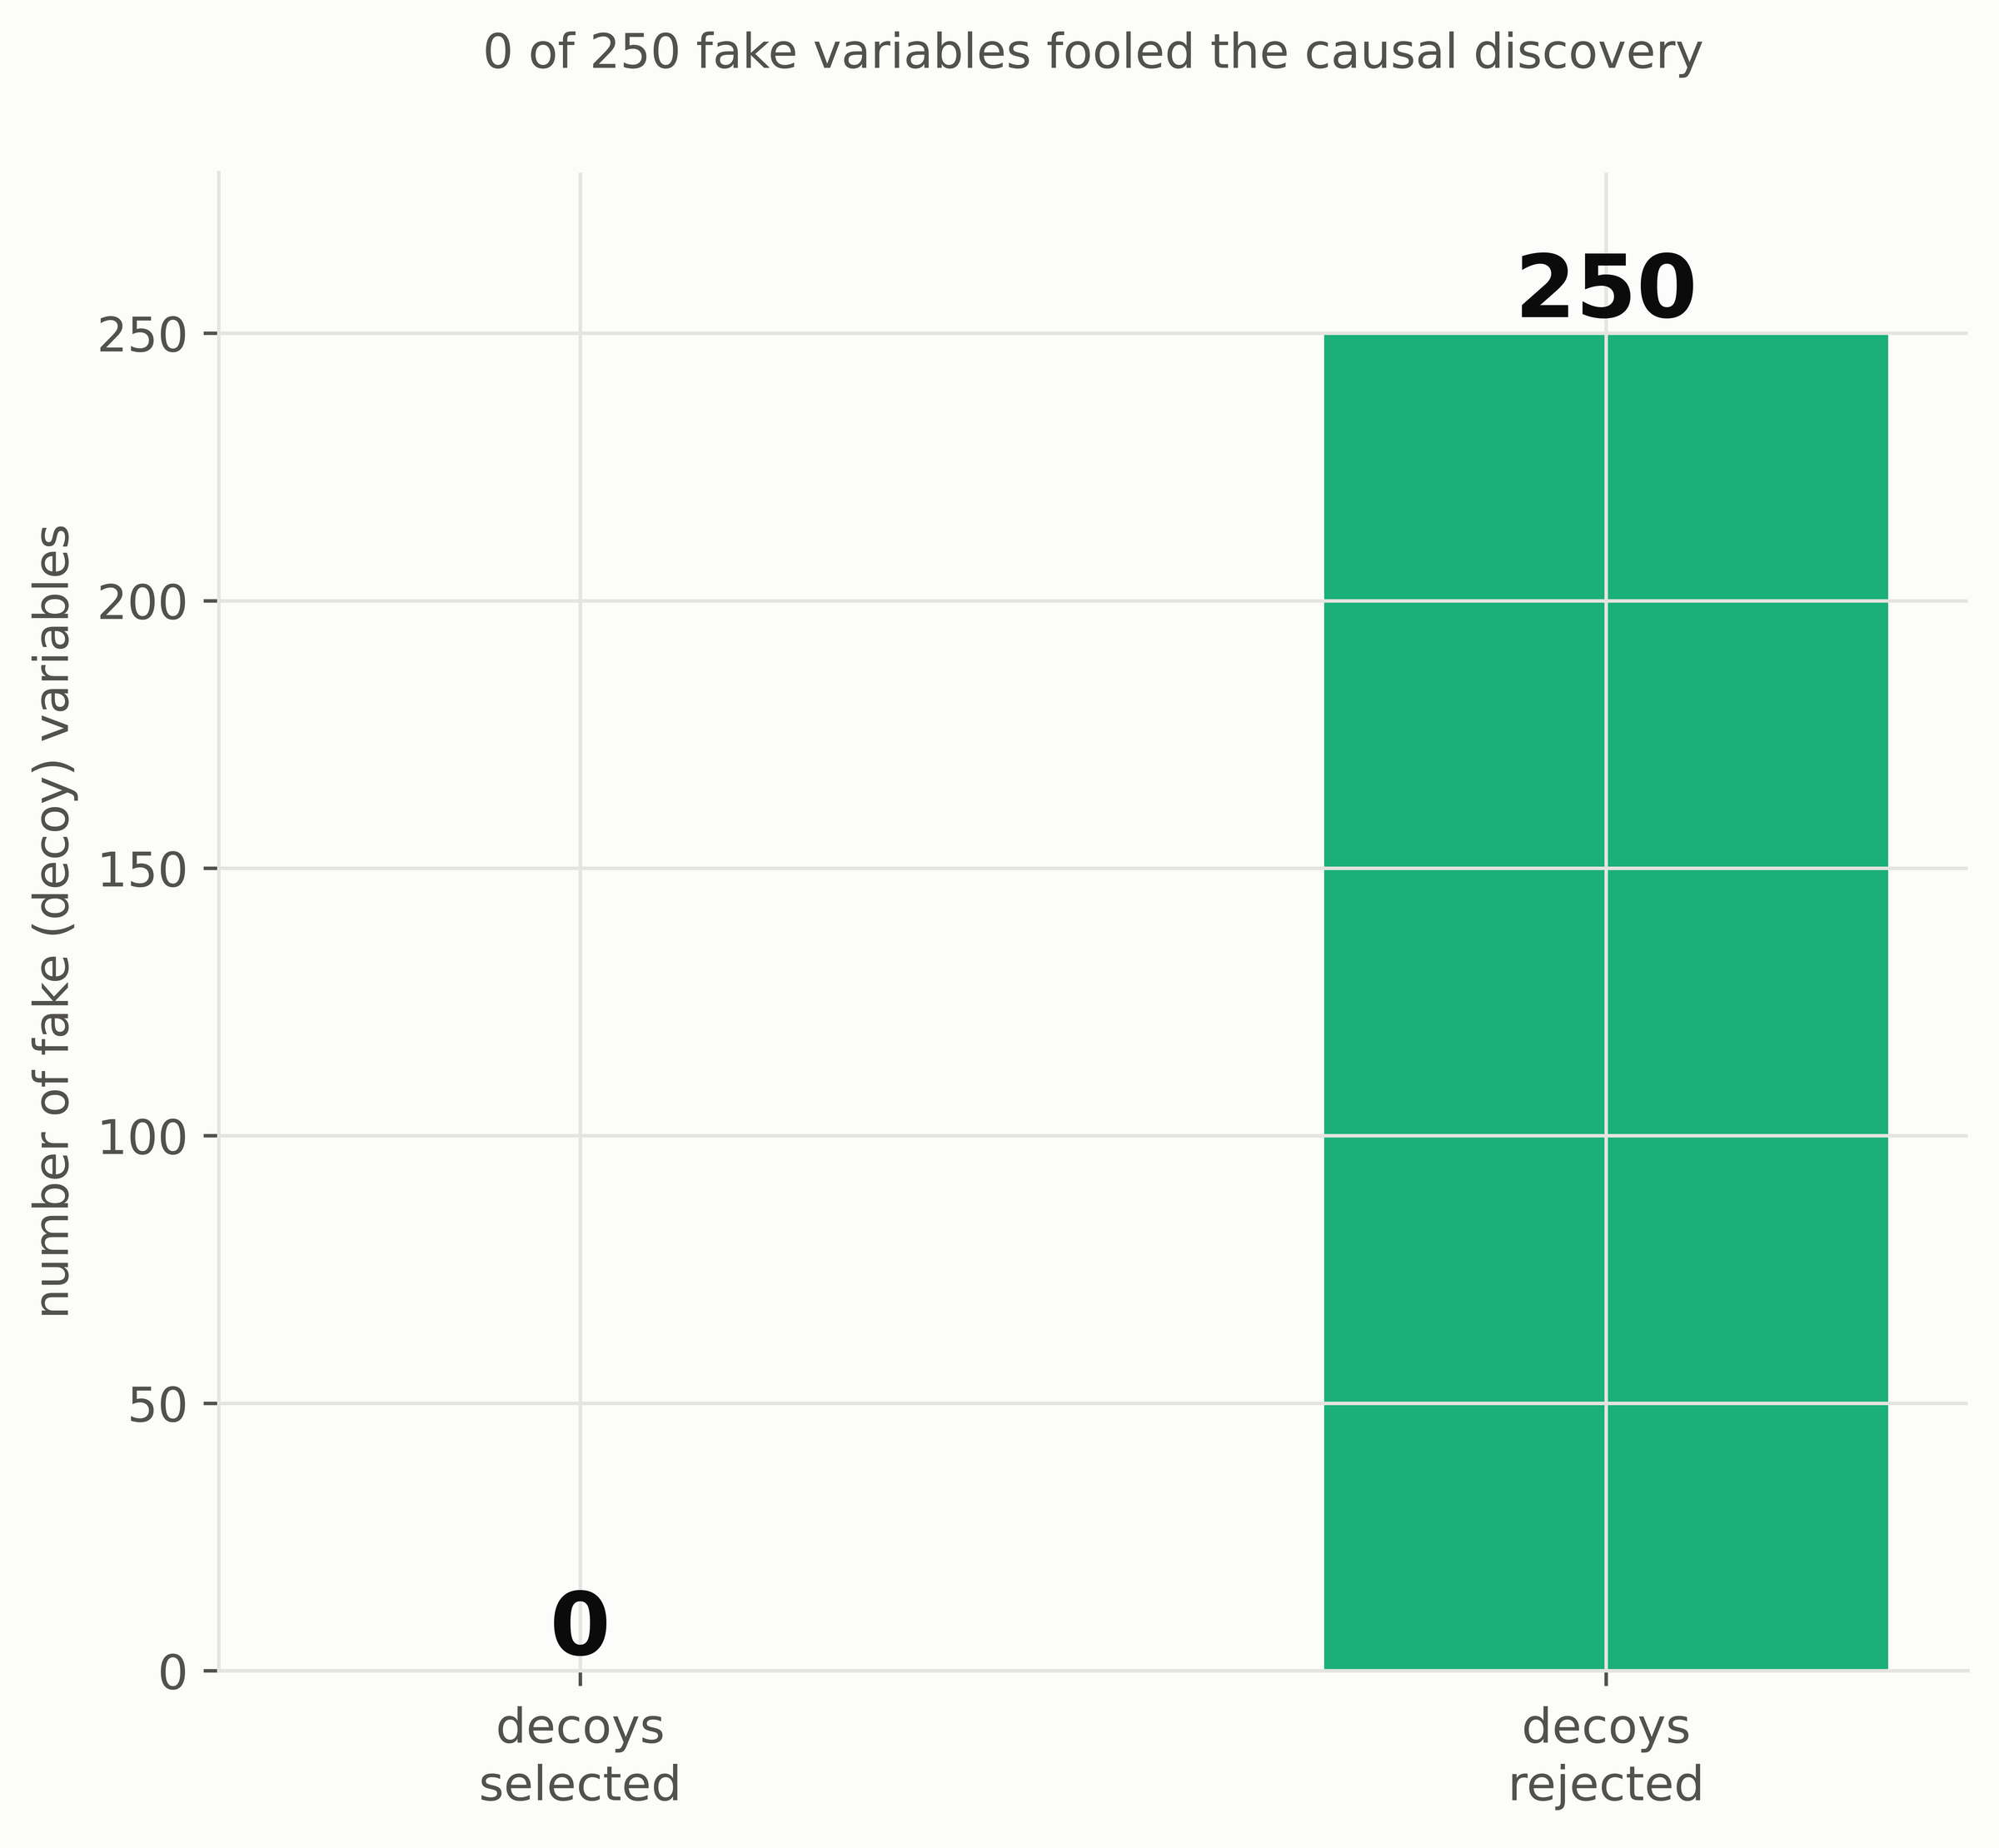
\includegraphics[width=\textwidth]{ppt_decoy_v1_big_count_bars.png}
\caption{B1: decoys selected vs rejected.}\label{fig:b1}
\end{subfigure}
\caption{The graph survives the first two checks almost unchanged. (a) Own-region links (blue) and outside links (orange) after each check. (b) None of the 250 phase-randomised decoys was selected as a parent of any target.}
\label{fig:b1b2}
\end{figure}

\paragraph{B1: decoys.} \textbf{None of the 250 decoys} was selected (decoy rate 0\%, against the 30\% warning line), while the real graph barely changed (517 real links in the decoy pass versus 536). The pipeline does not select series merely because they share the autocorrelation and the 30--60-day spectral peak of real climate nodes (Figures~\ref{fig:b1b2} and~\ref{fig:b1strength}).

\begin{figure}[htbp]
\centering
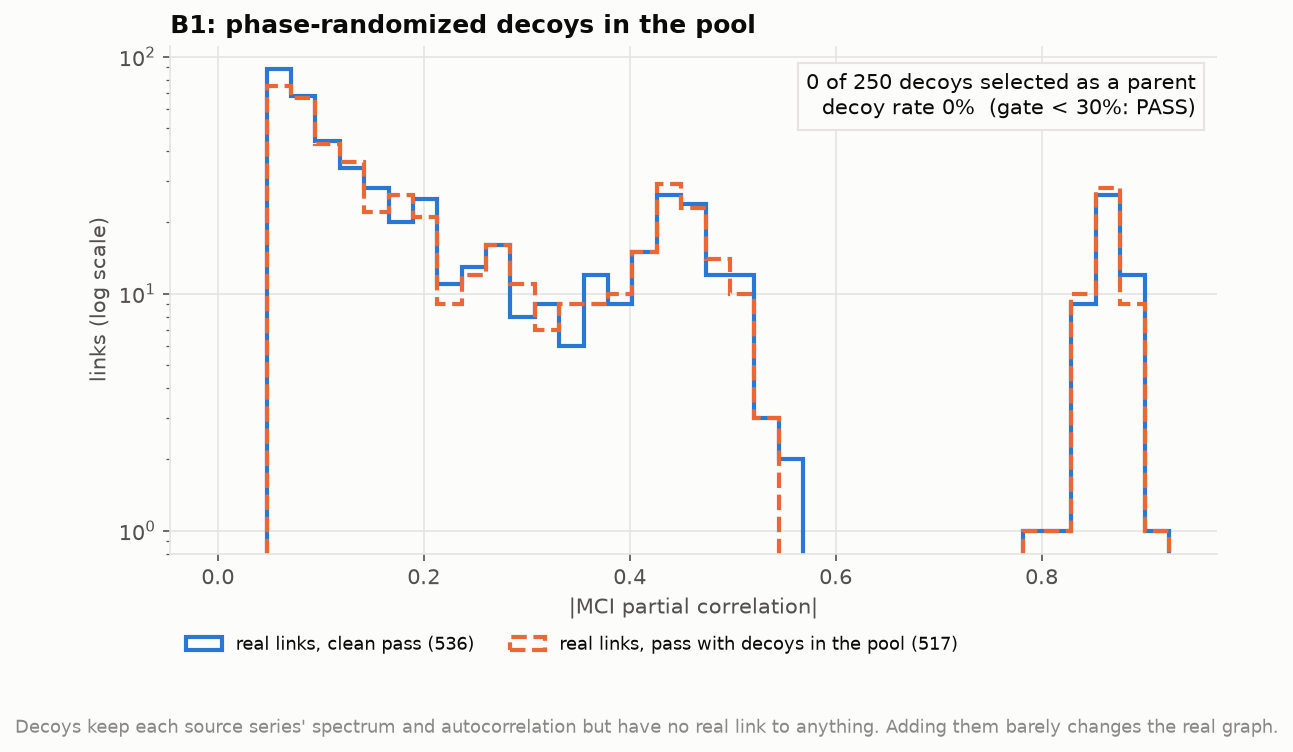
\includegraphics[width=0.7\textwidth]{04_b1_decoys.png}
\caption{B1: distribution of $|\hat\rho^{\,\mathrm{MCI}}|$ for real links in the clean pass (536) and in the pass with 250 decoys in the pool (517). The two distributions nearly coincide, including the strong own-OLR links near 0.85.}
\label{fig:b1strength}
\end{figure}

\paragraph{B2: physical lag mask.} Only \textbf{3 of 536} links need an impossible speed: h850 from region 22 to region 32 (5{,}531\,km at lag 1, 64\ms), and OLR from 28 to 33 (33\ms) and from 3 to 47 (26\ms). Of the outside links kept, 28 span 500--5{,}500\,km, and the fastest needs 46\ms; all of these come from wind and height fields, consistent with equatorial waves (Figure~\ref{fig:b2}). No link reaches the 25-day oscillation flag.

\begin{figure}[htbp]
\centering
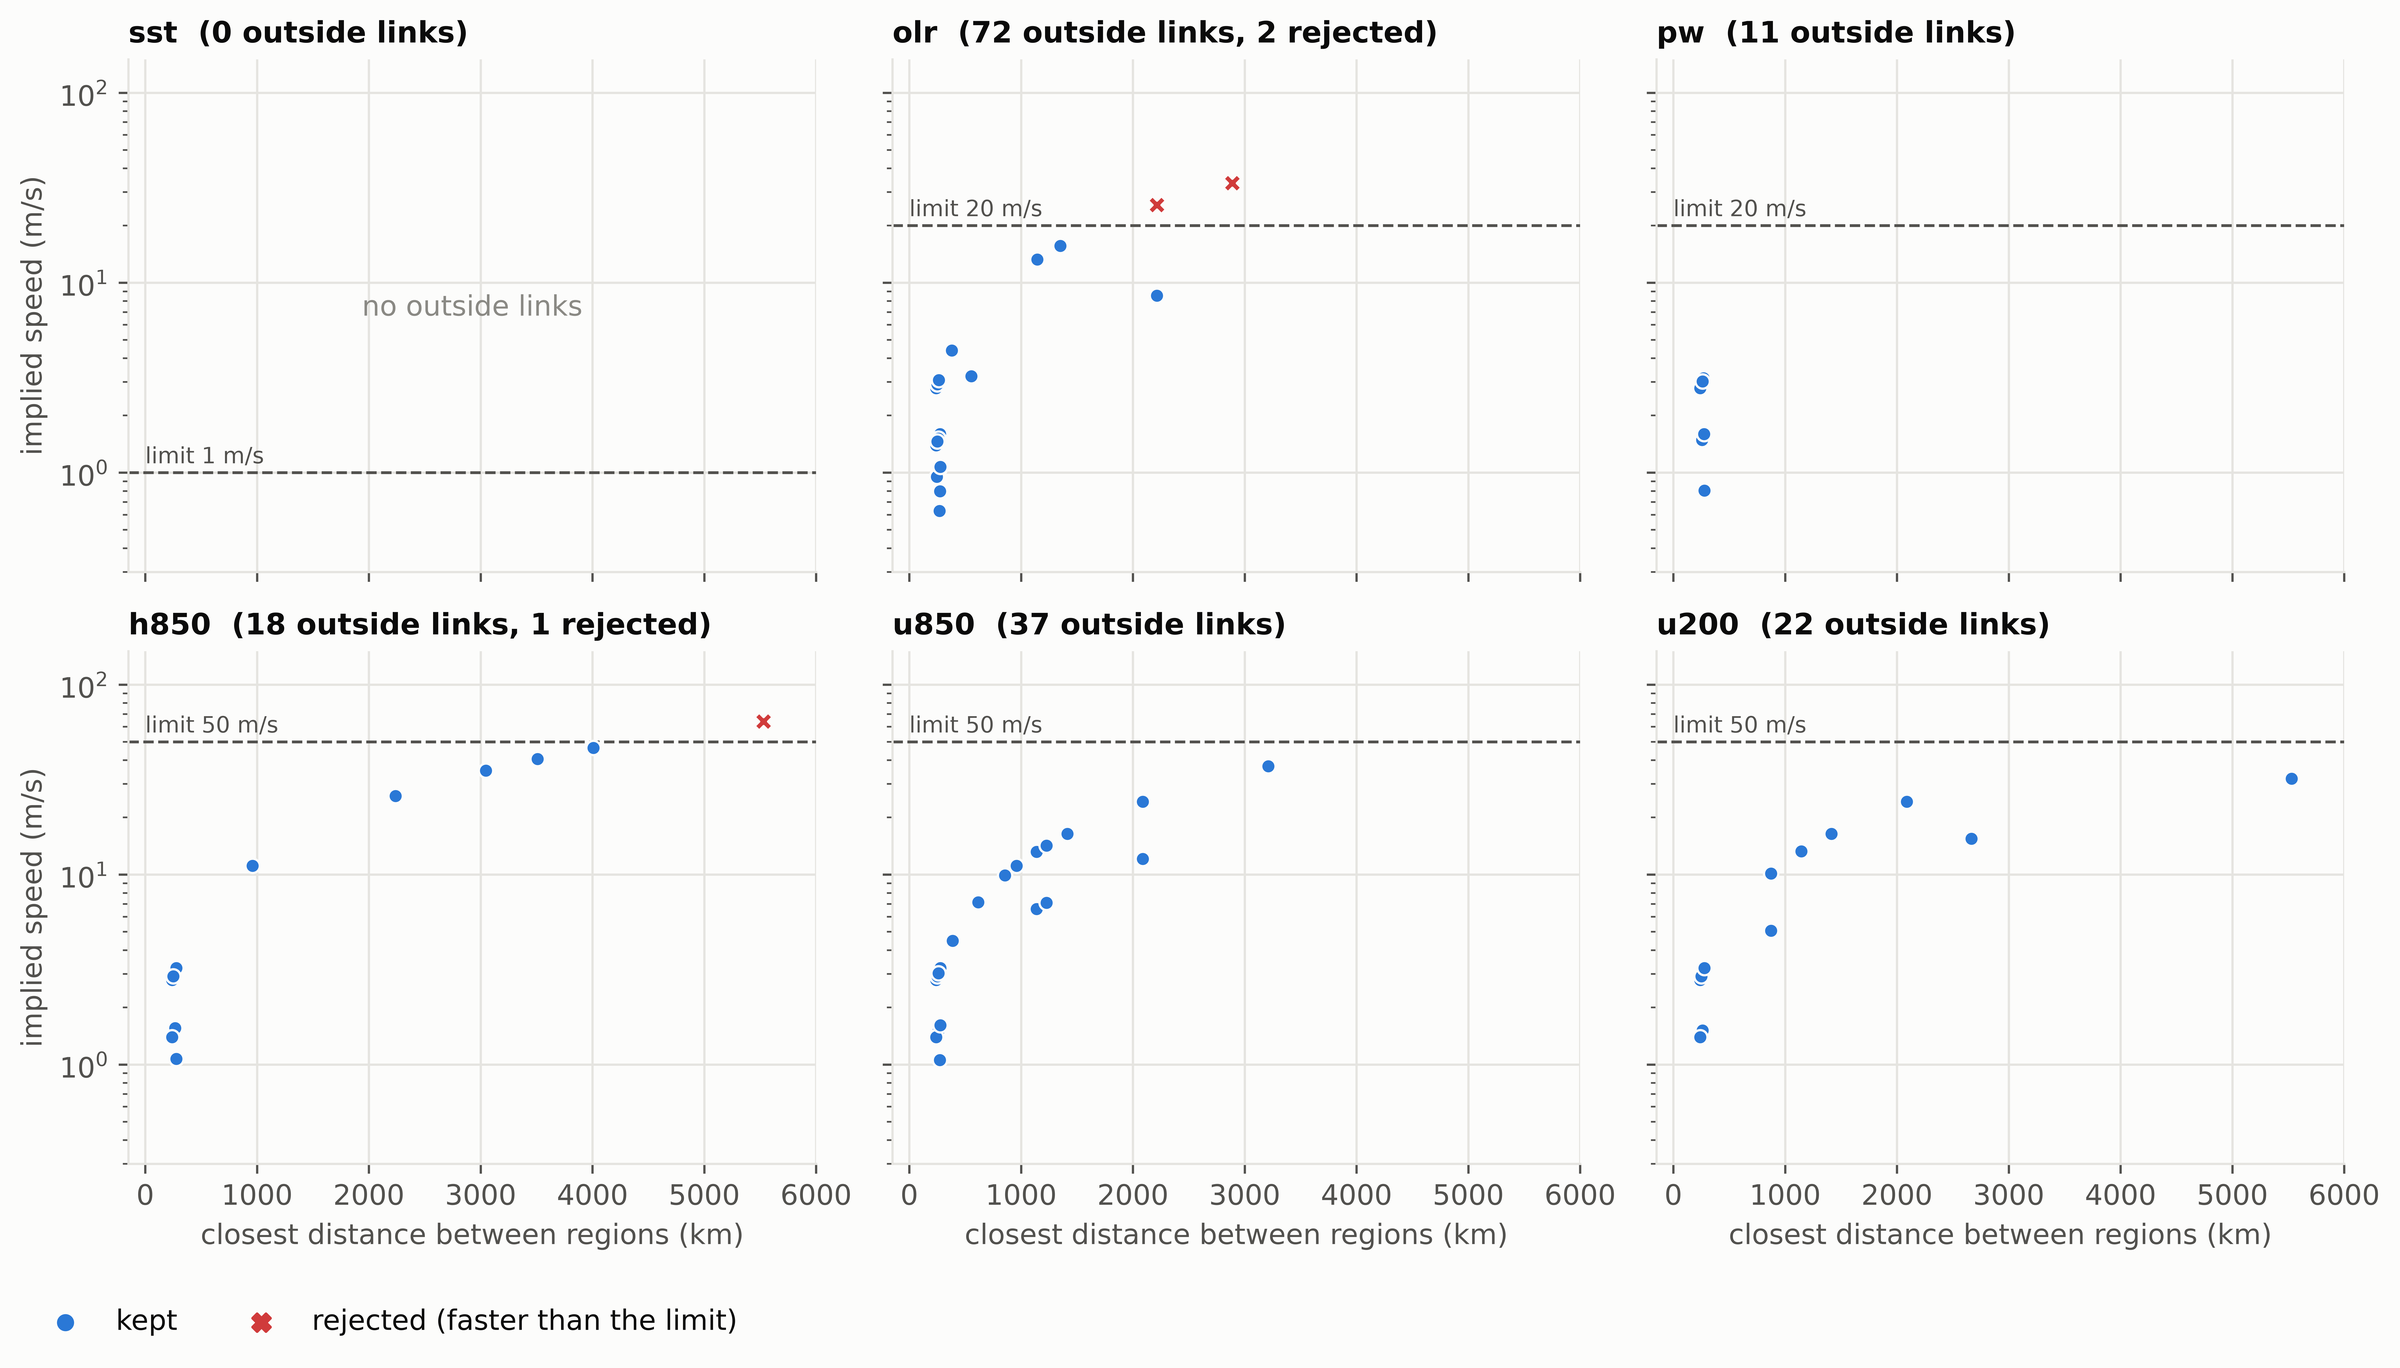
\includegraphics[width=\textwidth]{ppt_05b_b2_speed_no_title.png}
\caption{B2: implied speed against closest distance for every outside link, by source field, with each field's speed limit (dashed). Crosses are the three rejected links.}
\label{fig:b2}
\end{figure}

\paragraph{B3: top-$k$.} The validation $R^2$ rises from 0.9619 with own-region links only to 0.9633 with ten outside links, each extra link adding a little. The selected $k=10$ equals the largest number of outside links of any target, so all 157 surviving outside links are kept: PCMCI with FDR control is already sparse. The prior has \textbf{2.06 source regions per target}; two targets (regions 13 and 42) have no outside driver (Figure~\ref{fig:b3}).

\begin{figure}[htbp]
\centering
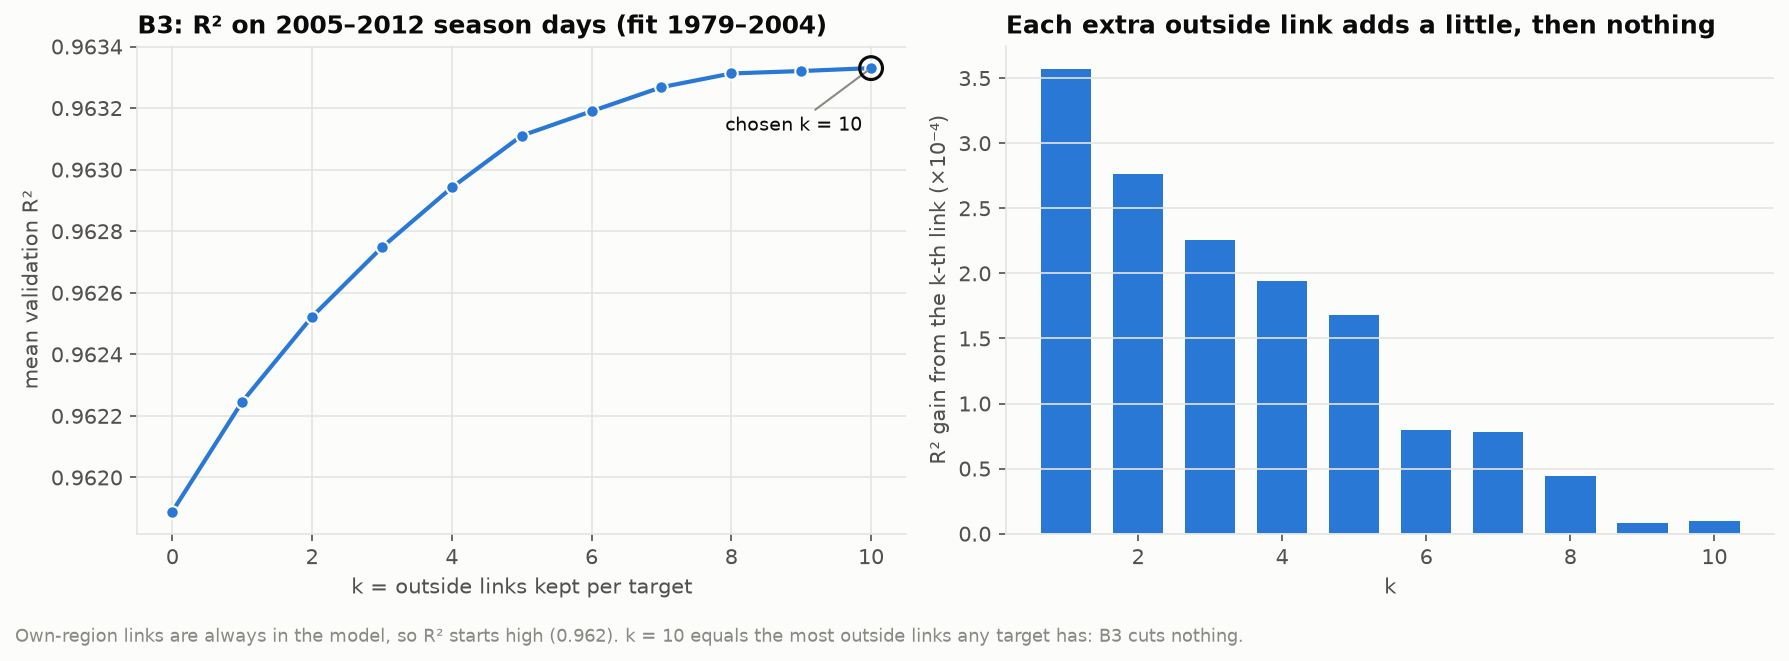
\includegraphics[width=\textwidth]{06_b3_k.png}
\caption{B3: mean validation $R^2$ on 2005--2012 season days against the number $k$ of outside links per target (left), and the gain from the $k$-th link (right).}
\label{fig:b3}
\end{figure}

\paragraph{B4: resolution persistence.} At 100 regions the mean persistence score is \textbf{0.62}, and \textbf{33 of 48} scored targets reach 0.5 (Figure~\ref{fig:b4}). OLR links persist best (56 of 70), followed by u200 (14 of 22); moisture and low-level height links, which are more local, persist least (PW 4 of 11, h850 6 of 17).

\begin{figure}[htbp]
\centering
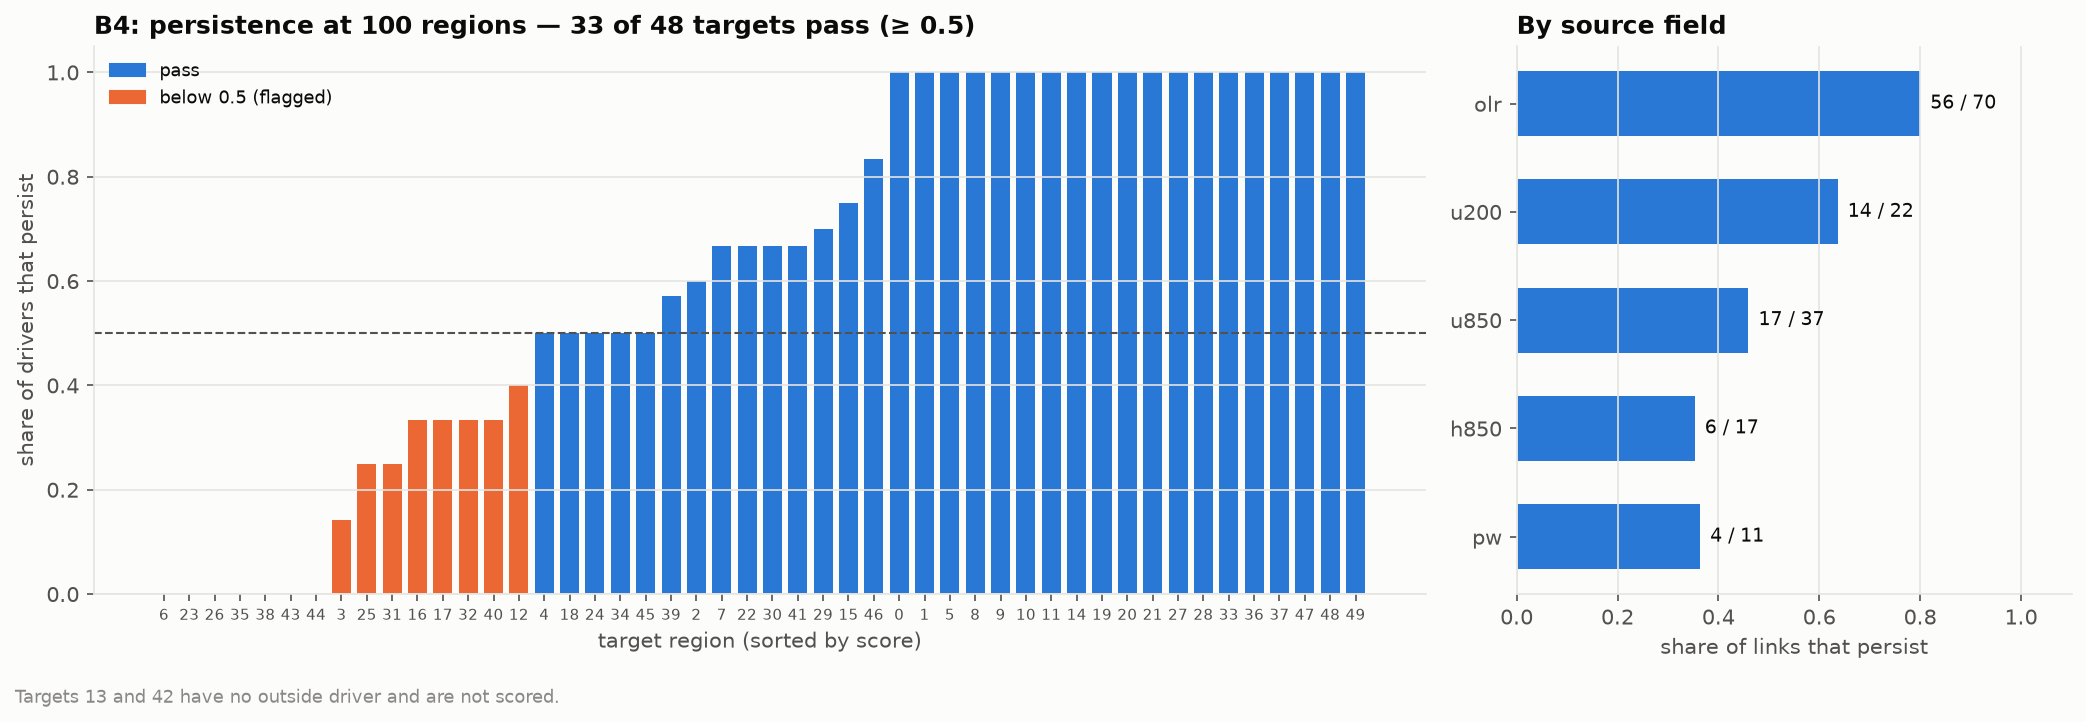
\includegraphics[width=\textwidth]{07_b4_persistence.png}
\caption{B4: persistence score of each target at 100 regions (left; orange below 0.5, flagged) and the share of links that persist by source field (right).}
\label{fig:b4}
\end{figure}

\noindent Hypotheses H1 and H2 are supported: the discovered graph is sparse, physically plausible and largely robust to the spatial partition.

\section{Source Selection and Forecasting (RQ3)}
\label{sec:res-stagec}

\subsection{The splitter without a prior}
\label{sec:res-pool}

Without a prior, the expert beats persistence at 7 days in all 50 regions in every candidate pool, with a mean skill of about $+0.40$. The year-round 7-day forecast in the direct pool has a mean MSE of 0.317 and a mean RMSE of 0.559 standard deviations (Figure~\ref{fig:mse}). Source discrimination, however, depends strongly on the pool (Table~\ref{tab:pool}): 27--30 regions have informative splitters in the direct pool, 8--9 in the 2hop pool, and none in the full pool. With 50 similar-looking candidates, the shared scoring network cannot separate them. Figure~\ref{fig:poolfig} shows the same contrast: accuracy is flat across pools while discrimination collapses. Discrimination also needs enough training: with the direct pool, 5 epochs give 27 informative regions against 5 after 2 epochs (Figure~\ref{fig:epochs}).

\begin{table}[htbp]
\centering
\caption{No-prior splitter by candidate pool, 7-day lead, 50 regions, test period 2013--2022.}
\label{tab:pool}
\footnotesize
\setlength{\tabcolsep}{3pt}
\begin{tabular}{llccc}
\toprule
\textbf{Target days} & \textbf{Pool} & \textbf{Informative splitters} & \textbf{Beat persistence} & \textbf{Mean $S_{\mathrm{pers}}$} \\
\midrule
Year-round & direct / 2hop / full & 27 / 8 / 0 & 50 / 50 / 50 & $+0.401$ / $+0.395$ / $+0.396$ \\
BSISO season & direct / 2hop / full & 30 / 9 / 0 & 50 / 50 / 50 & $+0.412$ / $+0.413$ / $+0.415$ \\
\bottomrule
\end{tabular}
\end{table}

\begin{figure}[htbp]
\centering
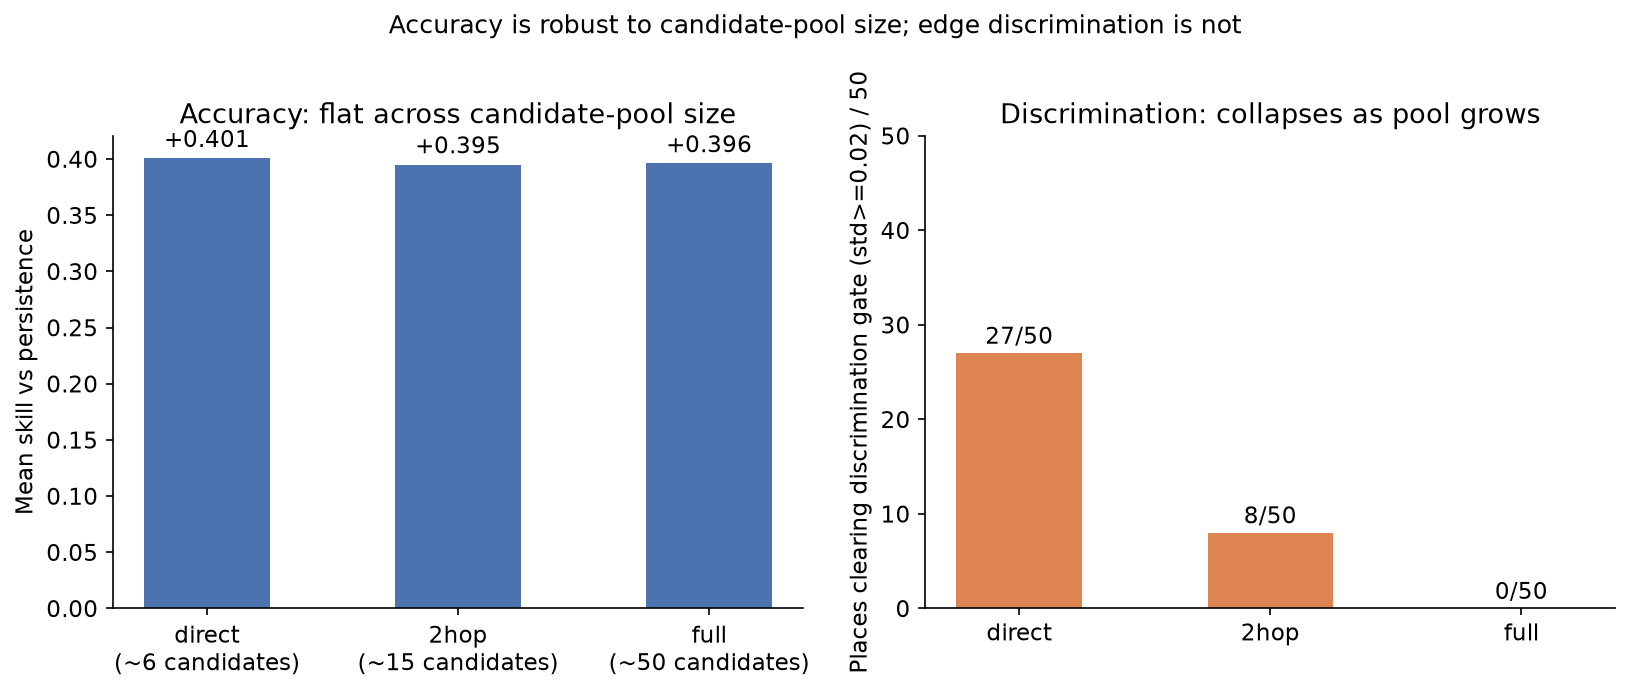
\includegraphics[width=0.85\textwidth]{02_variant_comparison.png}
\caption{No-prior splitter, year-round, 7-day lead: skill relative to persistence is flat across candidate pools (left), while the number of regions with informative splitter scores collapses as the pool grows (right).}
\label{fig:poolfig}
\end{figure}

\begin{figure}[htbp]
\centering
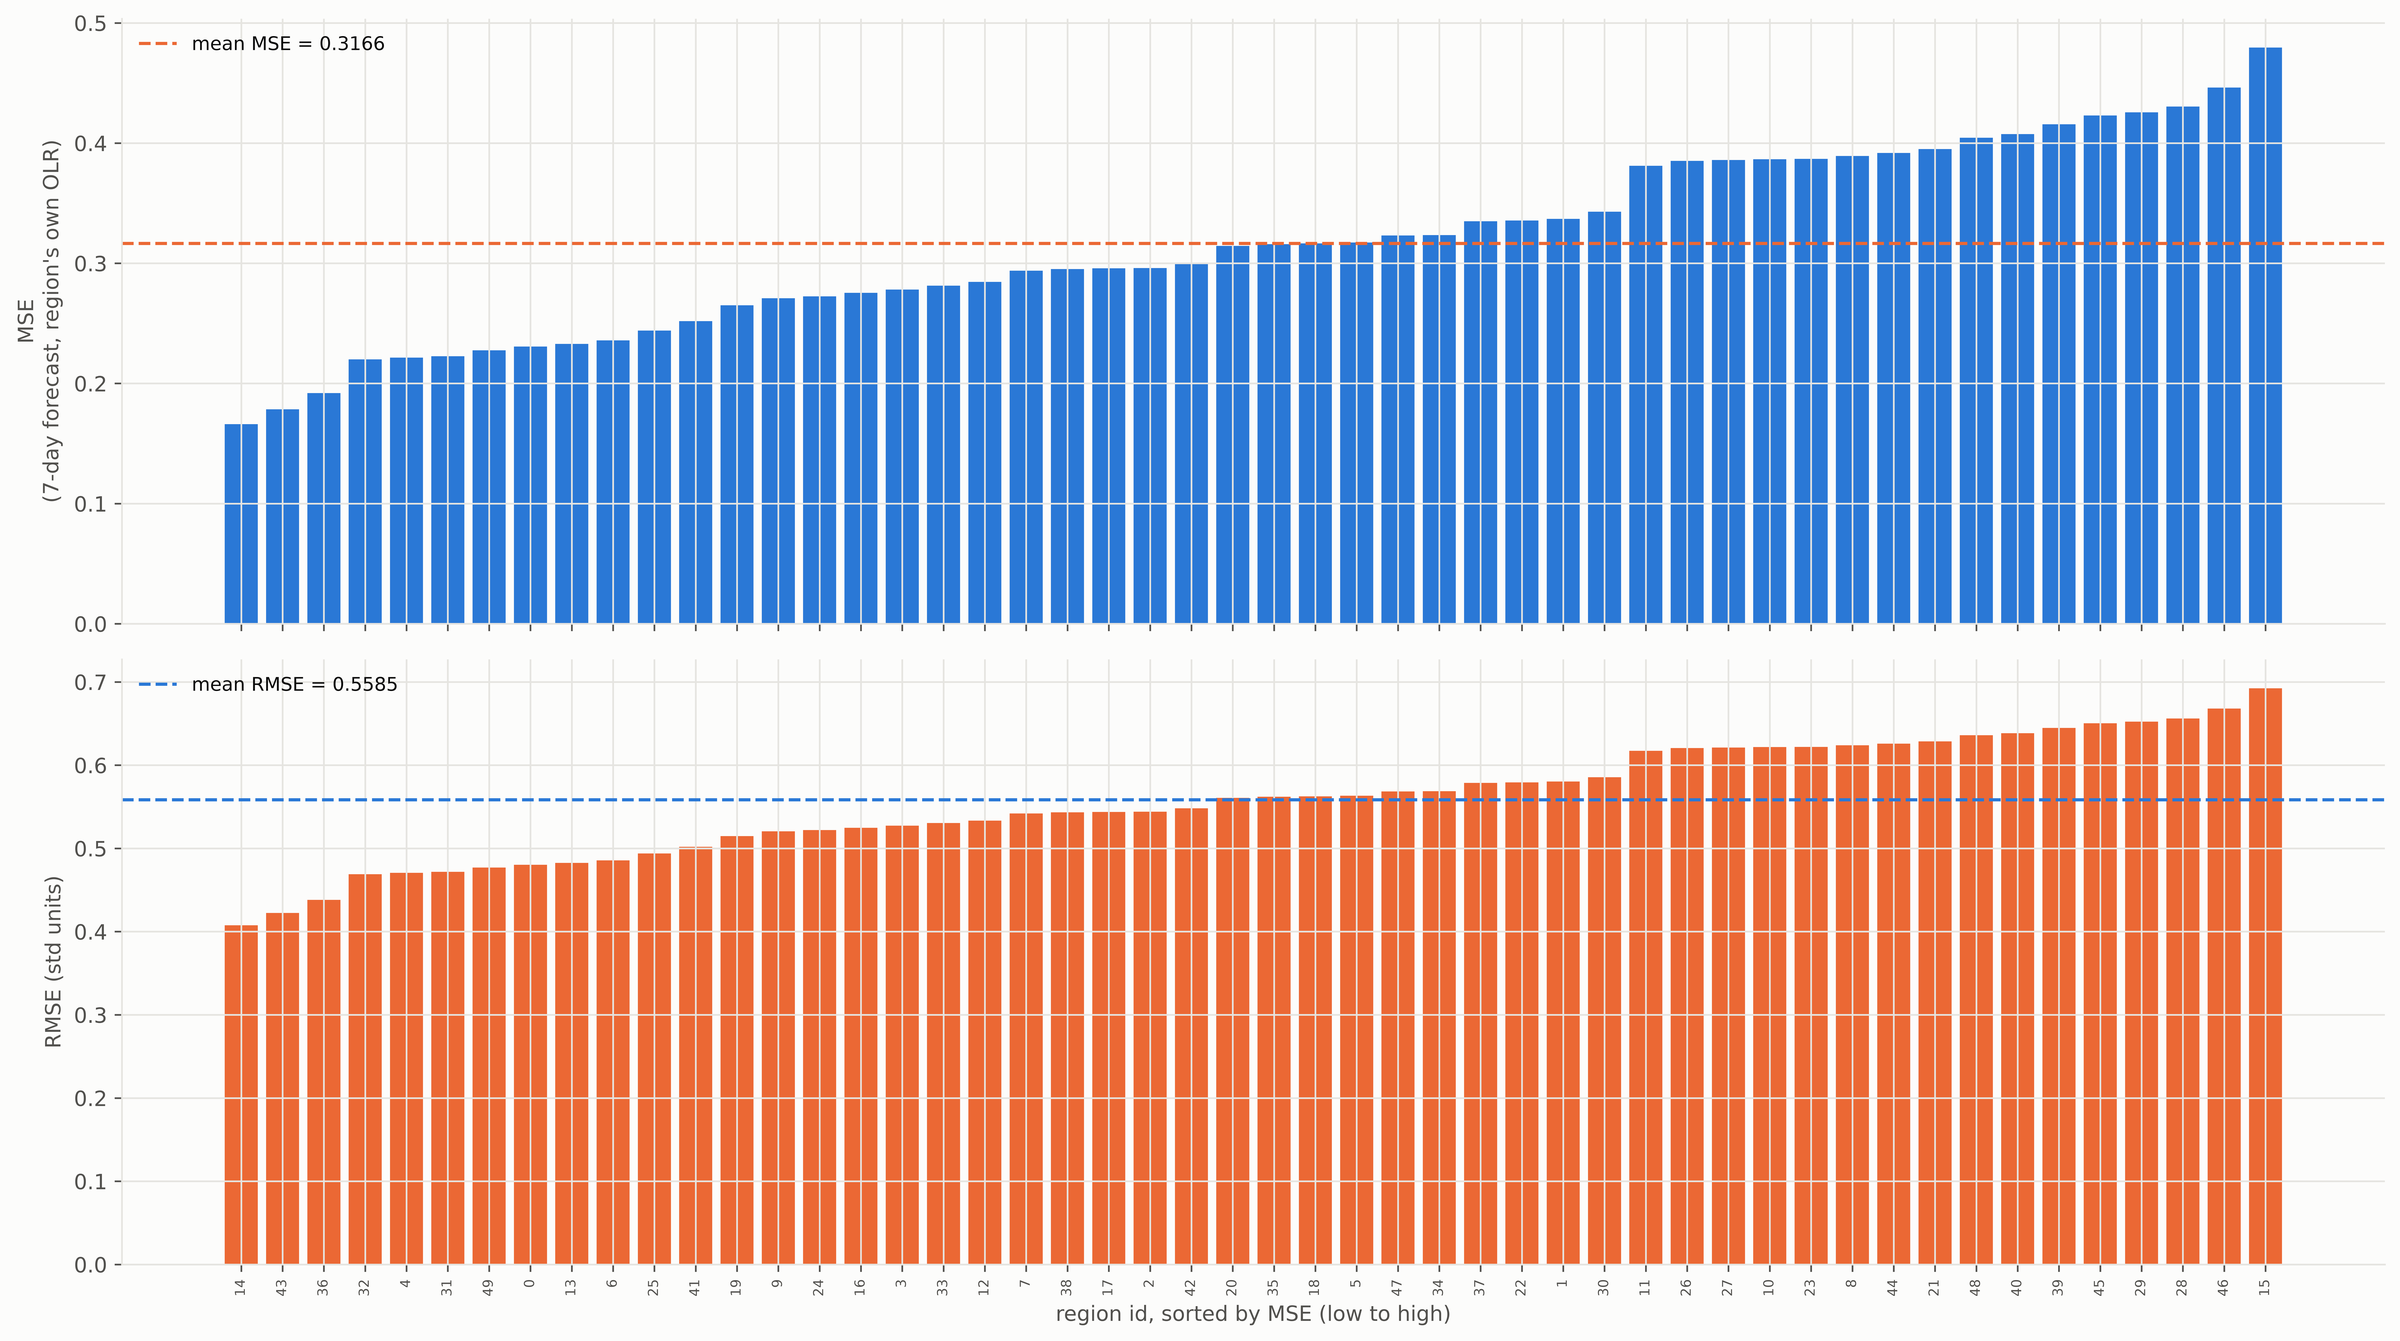
\includegraphics[width=\textwidth]{ppt_c3_per_region_mse_rmse_7day.png}
\caption{Per-region MSE (top) and RMSE (bottom) of the 7-day OLR forecast, direct pool, year-round test 2013--2022, sorted by error. Dashed lines: means (MSE 0.317, RMSE 0.559).}
\label{fig:mse}
\end{figure}

\begin{figure}[htbp]
\centering
\begin{subfigure}[b]{0.38\textwidth}\centering
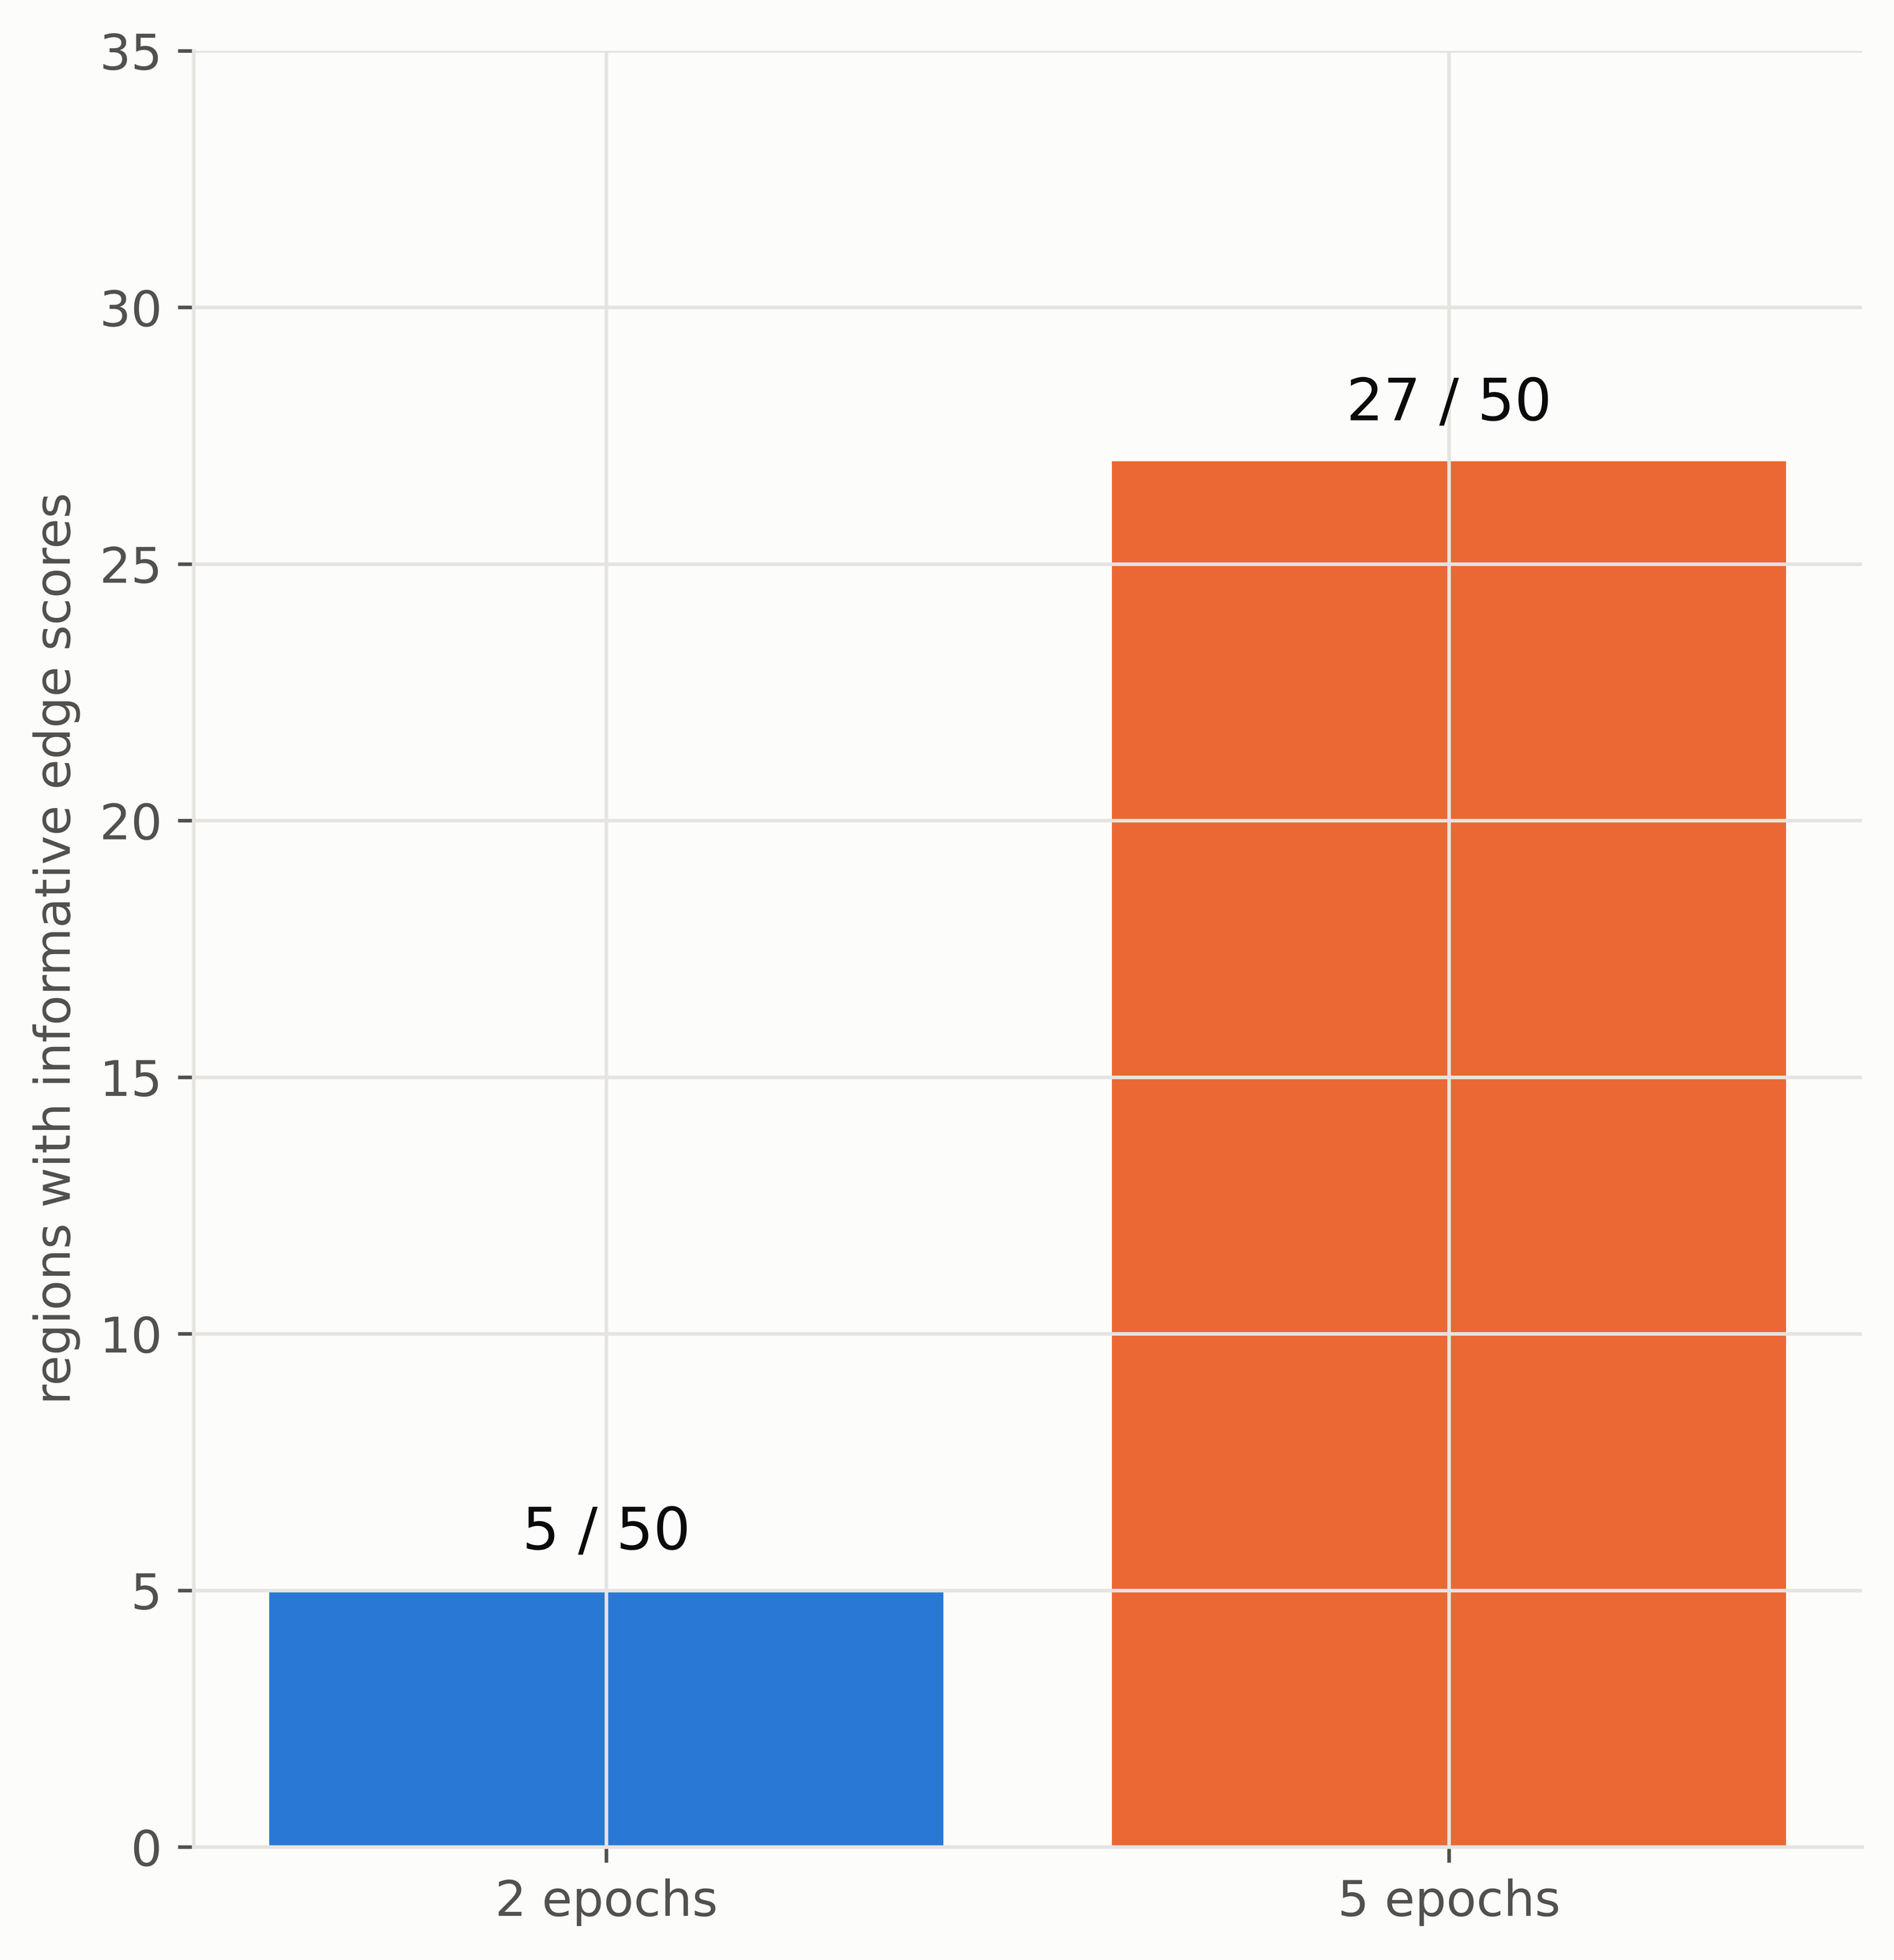
\includegraphics[width=\textwidth]{ppt_03c_informative_scores_2_vs_5_epochs.png}
\caption{Informative splitters, 2 vs 5 epochs.}\label{fig:epochs}
\end{subfigure}\hfill
\begin{subfigure}[b]{0.58\textwidth}\centering
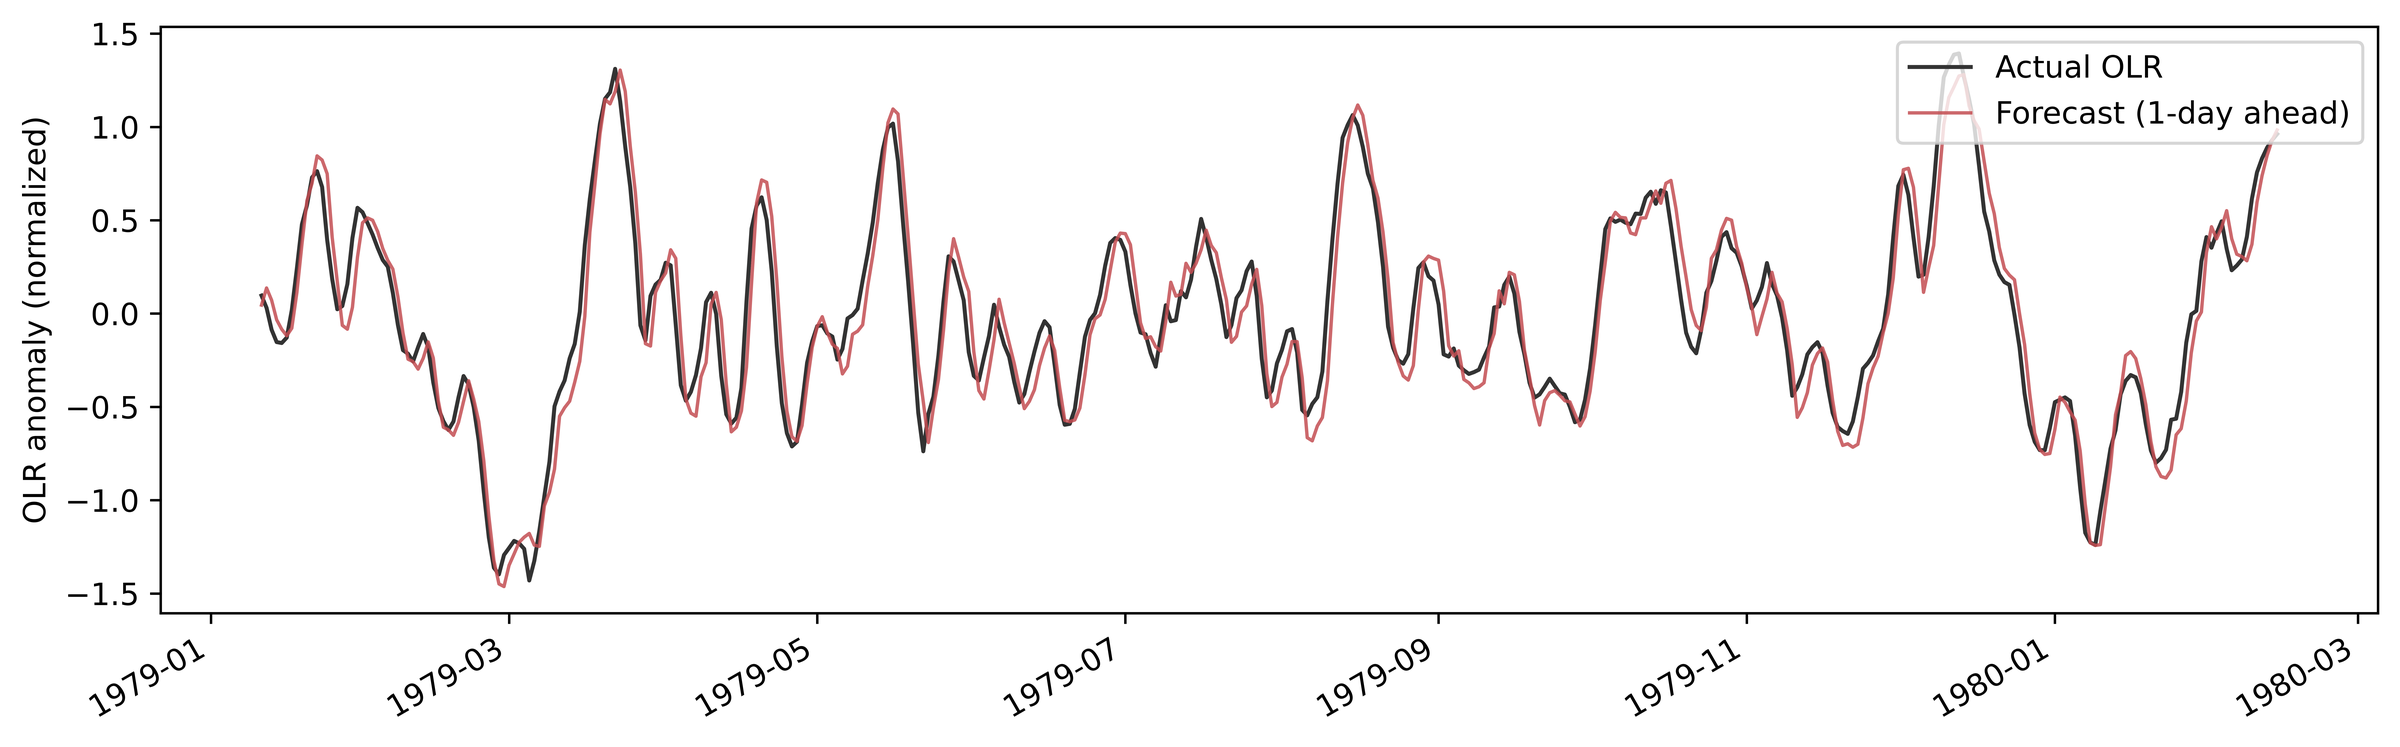
\includegraphics[width=\textwidth]{ppt_09_2_forecast_vs_actual_no_title.png}
\caption{Region 22, 1-day forecast vs observed OLR (illustrative 1979--80 window).}\label{fig:fva}
\end{subfigure}
\caption{(a) Splitter discrimination needs an adequate training budget. (b) The expert follows the observed OLR anomalies one day ahead, including sharp swings; held-out scores are reported in Table~\ref{tab:stagec}.}
\label{fig:epochs-fva}
\end{figure}

\subsection{The causal graph as a prior}

Table~\ref{tab:stagec} compares the PCMCI prior in restrict mode with no prior in the full pool on the 1{,}989 held-out season days.

\begin{table}[htbp]
\centering
\caption{PCMCI prior (restrict) vs no prior, full 50-region pool, 2013--2022 season days.}
\label{tab:stagec}
\footnotesize
\begin{tabular}{llccccc}
\toprule
\textbf{Lead} & \textbf{Prior} & \textbf{Informative} & \textbf{Beat pers.} & \textbf{Mean $S_{\mathrm{pers}}$} & \textbf{Beat clim.} & \textbf{Mean $R^2_{\mathrm{clim}}$} \\
\midrule
7 days & none & 0/50 & 50/50 & $+0.415$ & 14/50 & $-0.015$ \\
 & PCMCI & \textbf{24/50} & 50/50 & $+0.416$ & \textbf{19/50} & $-0.015$ \\
\midrule
1 day & none & 0/50 & 0/50 & $-1.527$ & 50/50 & $+0.720$ \\
 & PCMCI & \textbf{36/50} & 3/50 & $\mathbf{-1.327}$ & 50/50 & $\mathbf{+0.745}$ \\
\bottomrule
\end{tabular}
\end{table}

\paragraph{The prior makes source selection informative.} In the full pool, where the unguided splitter is uninformative in every region, the restrict prior yields informative splitters in 24 regions at 7 days and 36 at 1 day, without loss of accuracy.

\paragraph{One-day lead: skill improves.} The prior improves skill in \textbf{32 of 50 regions} (Figure~\ref{fig:stagec1}), with median gains of $+0.40$ in $S_{\mathrm{pers}}$ and $+0.048$ in $R^2_{\mathrm{clim}}$ (Wilcoxon $p=0.049$) and a median 17\% reduction in MSE. Region 22 improves from $S_{\mathrm{pers}}=-0.60$ to $-0.05$. Skill against persistence is negative at one day for both models because tomorrow's OLR is very close to today's; both are clearly skilful against climatology ($R^2_{\mathrm{clim}}>0.7$).

\begin{figure}[htbp]
\centering
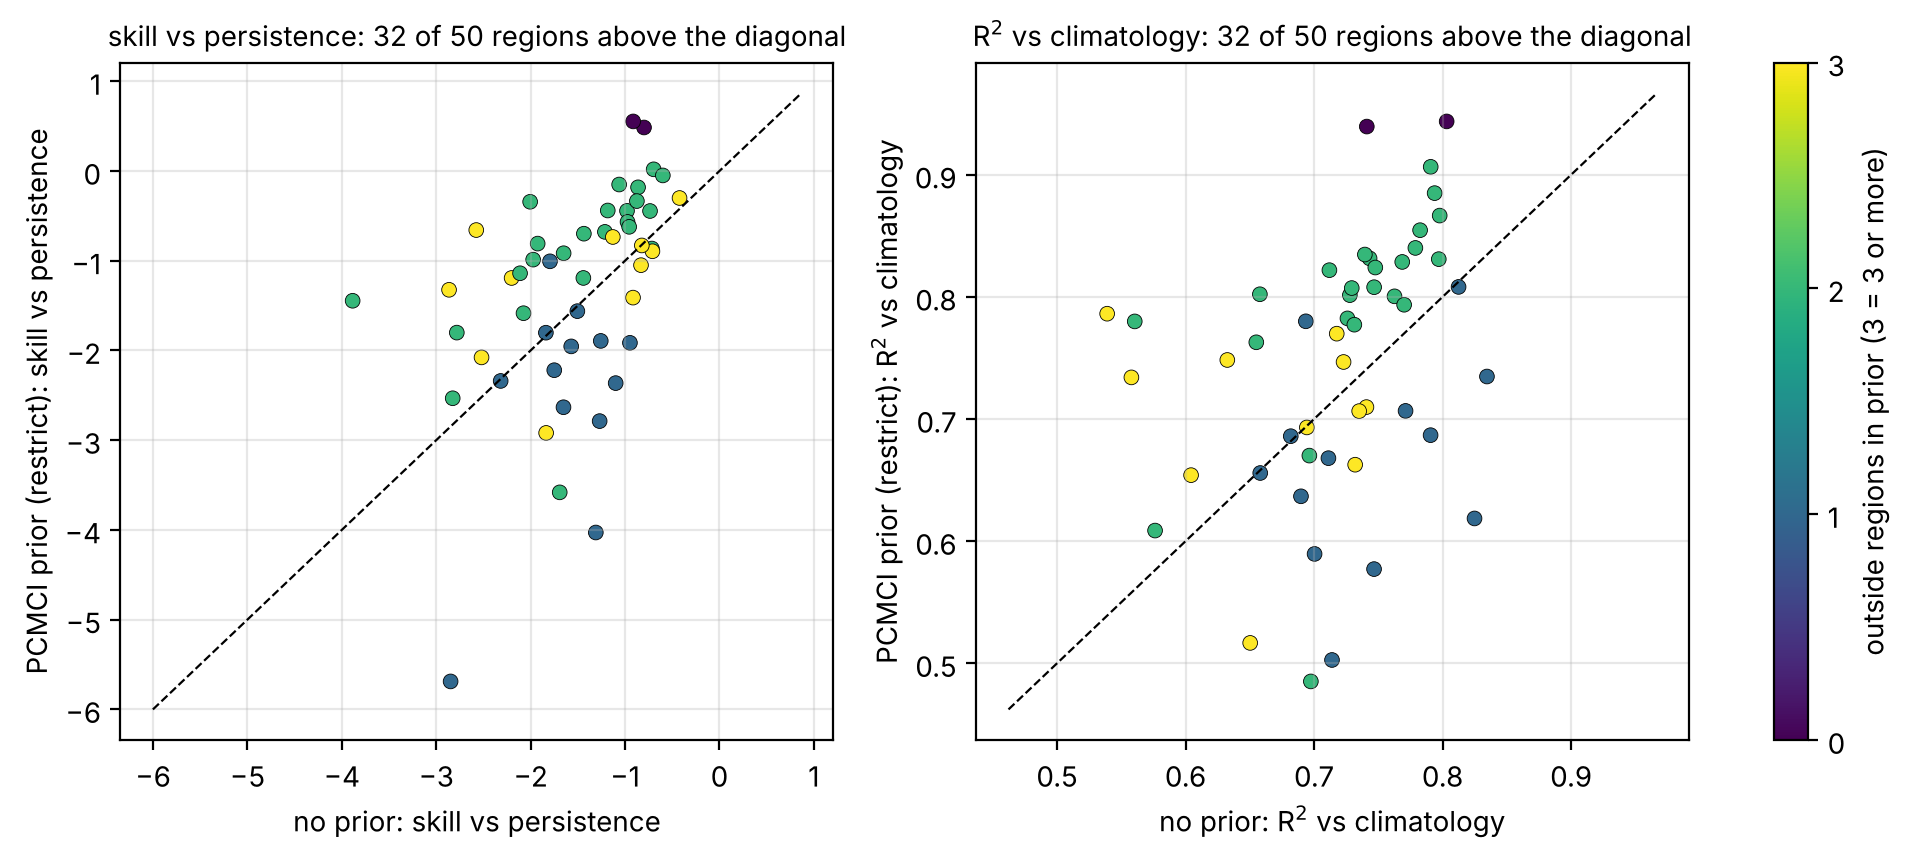
\includegraphics[width=0.92\textwidth]{10_stage_c_lead1.png}
\caption{One-day lead, full pool: per-region skill with the PCMCI prior against skill without a prior. Points above the diagonal improve; colour gives the number of outside regions in the prior.}
\label{fig:stagec1}
\end{figure}

\paragraph{Seven-day lead: unchanged.} At 7 days, skill is unchanged (23 regions better, 27 worse; mean $S_{\mathrm{pers}}$ $+0.416$ versus $+0.415$; Figure~\ref{fig:stagec7}), although 19 rather than 14 regions beat climatology. This follows from the graph's time scale: its outside links act within one or two days, so they describe exactly the information a 1-day forecast can use, but a source's state seven days before the target adds little. The graph identifies the right \emph{neighbours}, while a 7-day forecast needs week-ahead \emph{precursors}.

\begin{figure}[htbp]
\centering
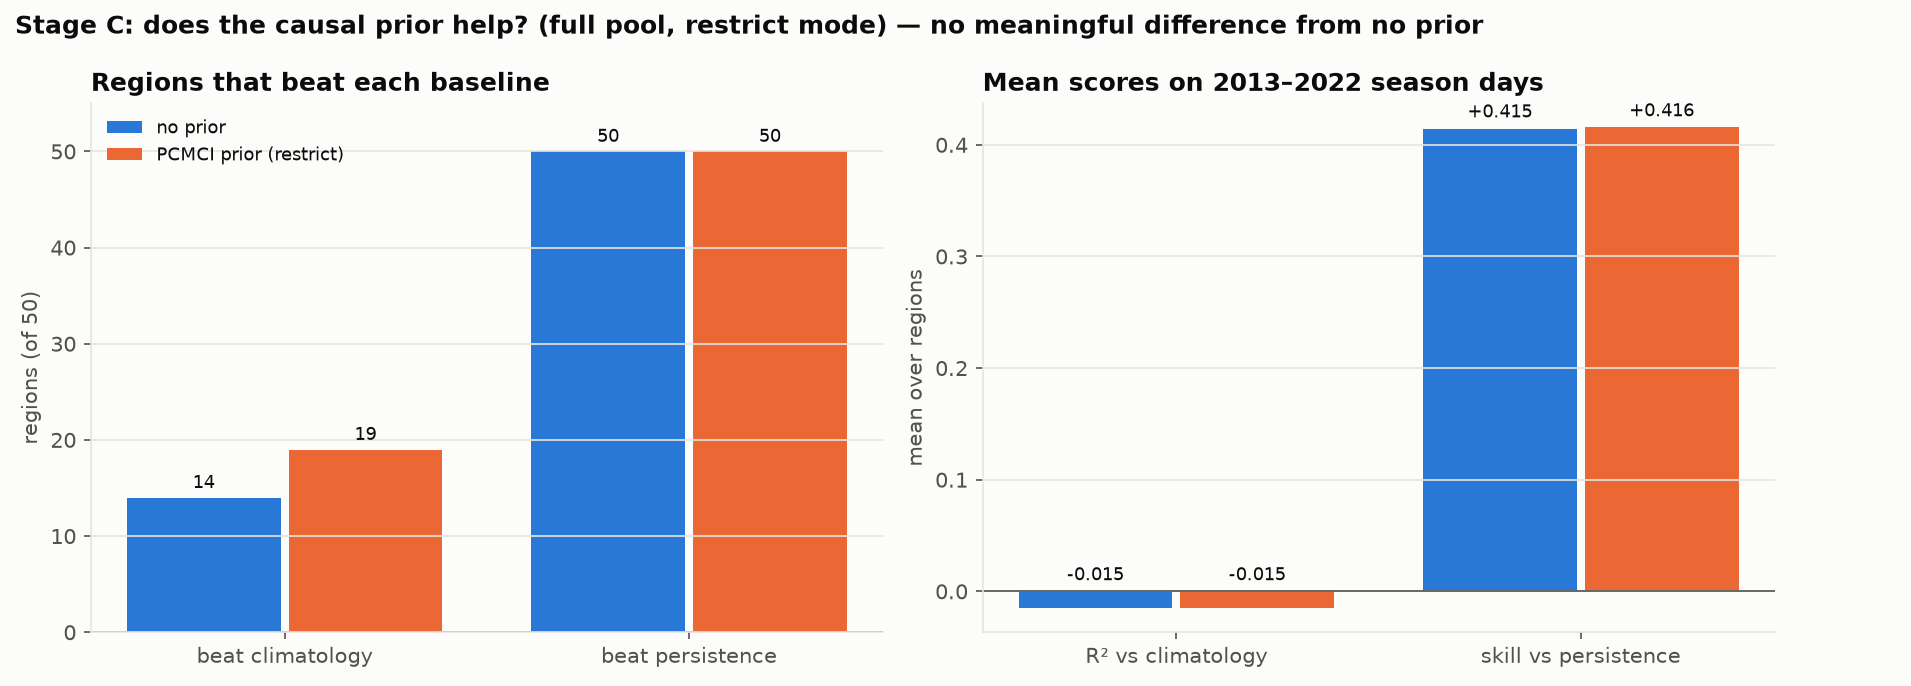
\includegraphics[width=0.92\textwidth]{09_stage_c_pcmci_vs_none.png}
\caption{Seven-day lead, full pool: regions beating each baseline (left) and mean scores (right), with and without the PCMCI restrict prior.}
\label{fig:stagec7}
\end{figure}

\paragraph{Dependence on prior size.} The one-day gain varies with prior size. The two targets with an empty prior, which are restricted to their own region, improve most ($S_{\mathrm{pers}}$ from $-0.86$ to $+0.52$); targets with two or more prior regions improve on average ($-1.53\to-0.91$ for two, $-1.53\to-1.22$ for three or more); and targets with a single prior region worsen ($-1.63\to-2.48$), because the splitter must then choose between the target's own history and its single driver. Comparing with random priors of equal size, the next step of the experimental programme, will separate the contribution of the graph's choice of regions from that of the smaller pool.

\section{Drift Detection (RQ4)}
\label{sec:res-drift}

Table~\ref{tab:drift} reports the four detector settings on an abrupt shift (the 1997--98 El Ni\~{n}o) and a gradual shift (2013--2022) at three regions.

\begin{table}[htbp]
\centering
\caption{Drift detection latency (days from the start of the shift window to the first alarm in it) and false-alarm rate (alarms per year outside all known shift events).}
\label{tab:drift}
\scriptsize
\setlength{\tabcolsep}{3.5pt}
\begin{tabular}{llcccc}
\toprule
\textbf{Region} & \textbf{Shift} & \textbf{Ch.\,1 error} & \textbf{Ch.\,2 structure} & \textbf{Fused OR} & \textbf{Fused AND} \\
\midrule
22 & abrupt 1997--98 & 159 d & \textbf{35 d} & 35 d & missed \\
   & gradual 2013--22 & 966 d & \textbf{181 d} & 181 d & 966 d \\
29 & abrupt 1997--98 & 223 d & \textbf{92 d} & 92 d & 235 d \\
   & gradual 2013--22 & 1{,}158 d & \textbf{117 d} & 117 d & 1{,}195 d \\
12 & abrupt 1997--98 & \textbf{95 d} & 123 d & 95 d & 123 d \\
   & gradual 2013--22 & \textbf{70 d} & 100 d & 70 d & 100 d \\
\midrule
\multicolumn{2}{l}{False alarms per year (22 / 29 / 12)} & 0.17 / 0.34 / 1.04 & 1.62 / 2.25 / 2.19 & 1.78 / 2.59 / 3.23 & 0.17 / 0.34 / 0.94 \\
\bottomrule
\end{tabular}
\end{table}

All shifts are detected by the OR fusion at every region. At regions 22 and 29 the causal-structure channel detects the abrupt El Ni\~{n}o shift 2.4--4.5 times sooner than the error channel, and the gradual shift 5.3--9.9 times sooner, which supports H4: watching the causal structure can reveal a change before it shows in the forecast error. At region 12 the error channel is faster. The structure channel raises more false alarms, so the fusion rule is a genuine trade-off between speed (OR) and caution (AND).

\section{Expert Lifecycle (RQ4)}
\label{sec:res-lifecycle}

Over 1979--2022, the lifecycle handled 49--61 regime changes per region. In \textbf{104 of 171} (61\%) an archived expert matched the new regime and was reactivated instead of a fresh expert being trained (Figure~\ref{fig:timeline}): regimes recur, and the archive reuses what was learned about them, supporting H5.

\begin{figure}[htbp]
\centering
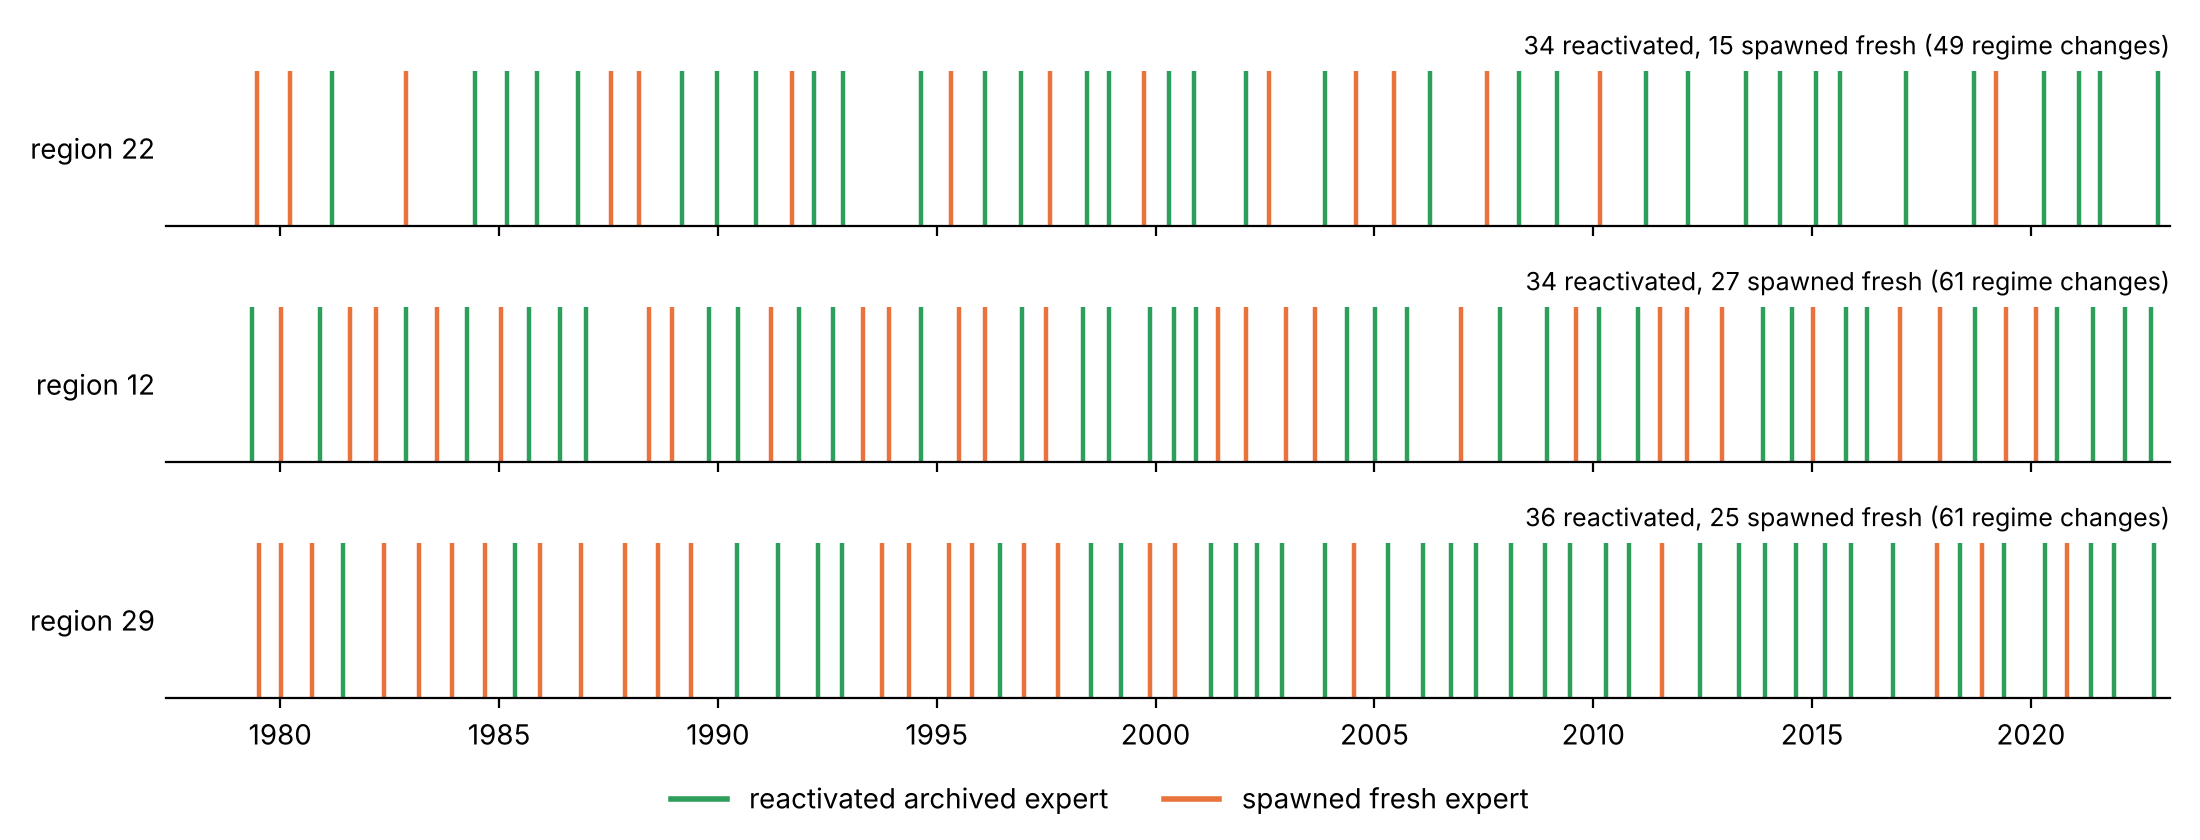
\includegraphics[width=\textwidth]{11_lifecycle_timeline.png}
\caption{Expert lifecycle events, 1979--2022: reactivation of an archived expert (green) or spawning of a fresh expert (orange) at each detected regime change, for regions 22, 12 and 29.}
\label{fig:timeline}
\end{figure}

\begin{table}[htbp]
\centering
\caption{Reactivation strategies: single best-matching archived expert vs a similarity-weighted blend of the top three.}
\label{tab:pool-blend}
\footnotesize
\begin{tabular}{lccc}
\toprule
 & \textbf{Region 22} & \textbf{Region 12} & \textbf{Region 29} \\
\midrule
Blend beats single (events) & 30/49 (61\%) & 42/61 (69\%) & 41/61 (67\%) \\
Mean MSE: single $\to$ blend & 0.368 $\to$ \textbf{0.352} & 0.422 $\to$ \textbf{0.402} & 0.384 $\to$ \textbf{0.376} \\
Forgetting: single $\to$ blend & $-0.010\to\mathbf{-0.013}$ & $0.183\to\mathbf{0.170}$ & $0.092\to\mathbf{0.086}$ \\
\bottomrule
\end{tabular}
\end{table}

Blending the three most similar archived experts beats reactivating the single best match on both forecast error and forgetting at all three regions (Table~\ref{tab:pool-blend}). Whether a reactivated expert should be warm-started from its archived weights or trained fresh depends on the region (Figure~\ref{fig:forget}): warm-starting gives lower forecast error in 28 of 34 events at region 22 and 24 of 36 at region 29, but lower forgetting only at region 29.

\begin{figure}[htbp]
\centering
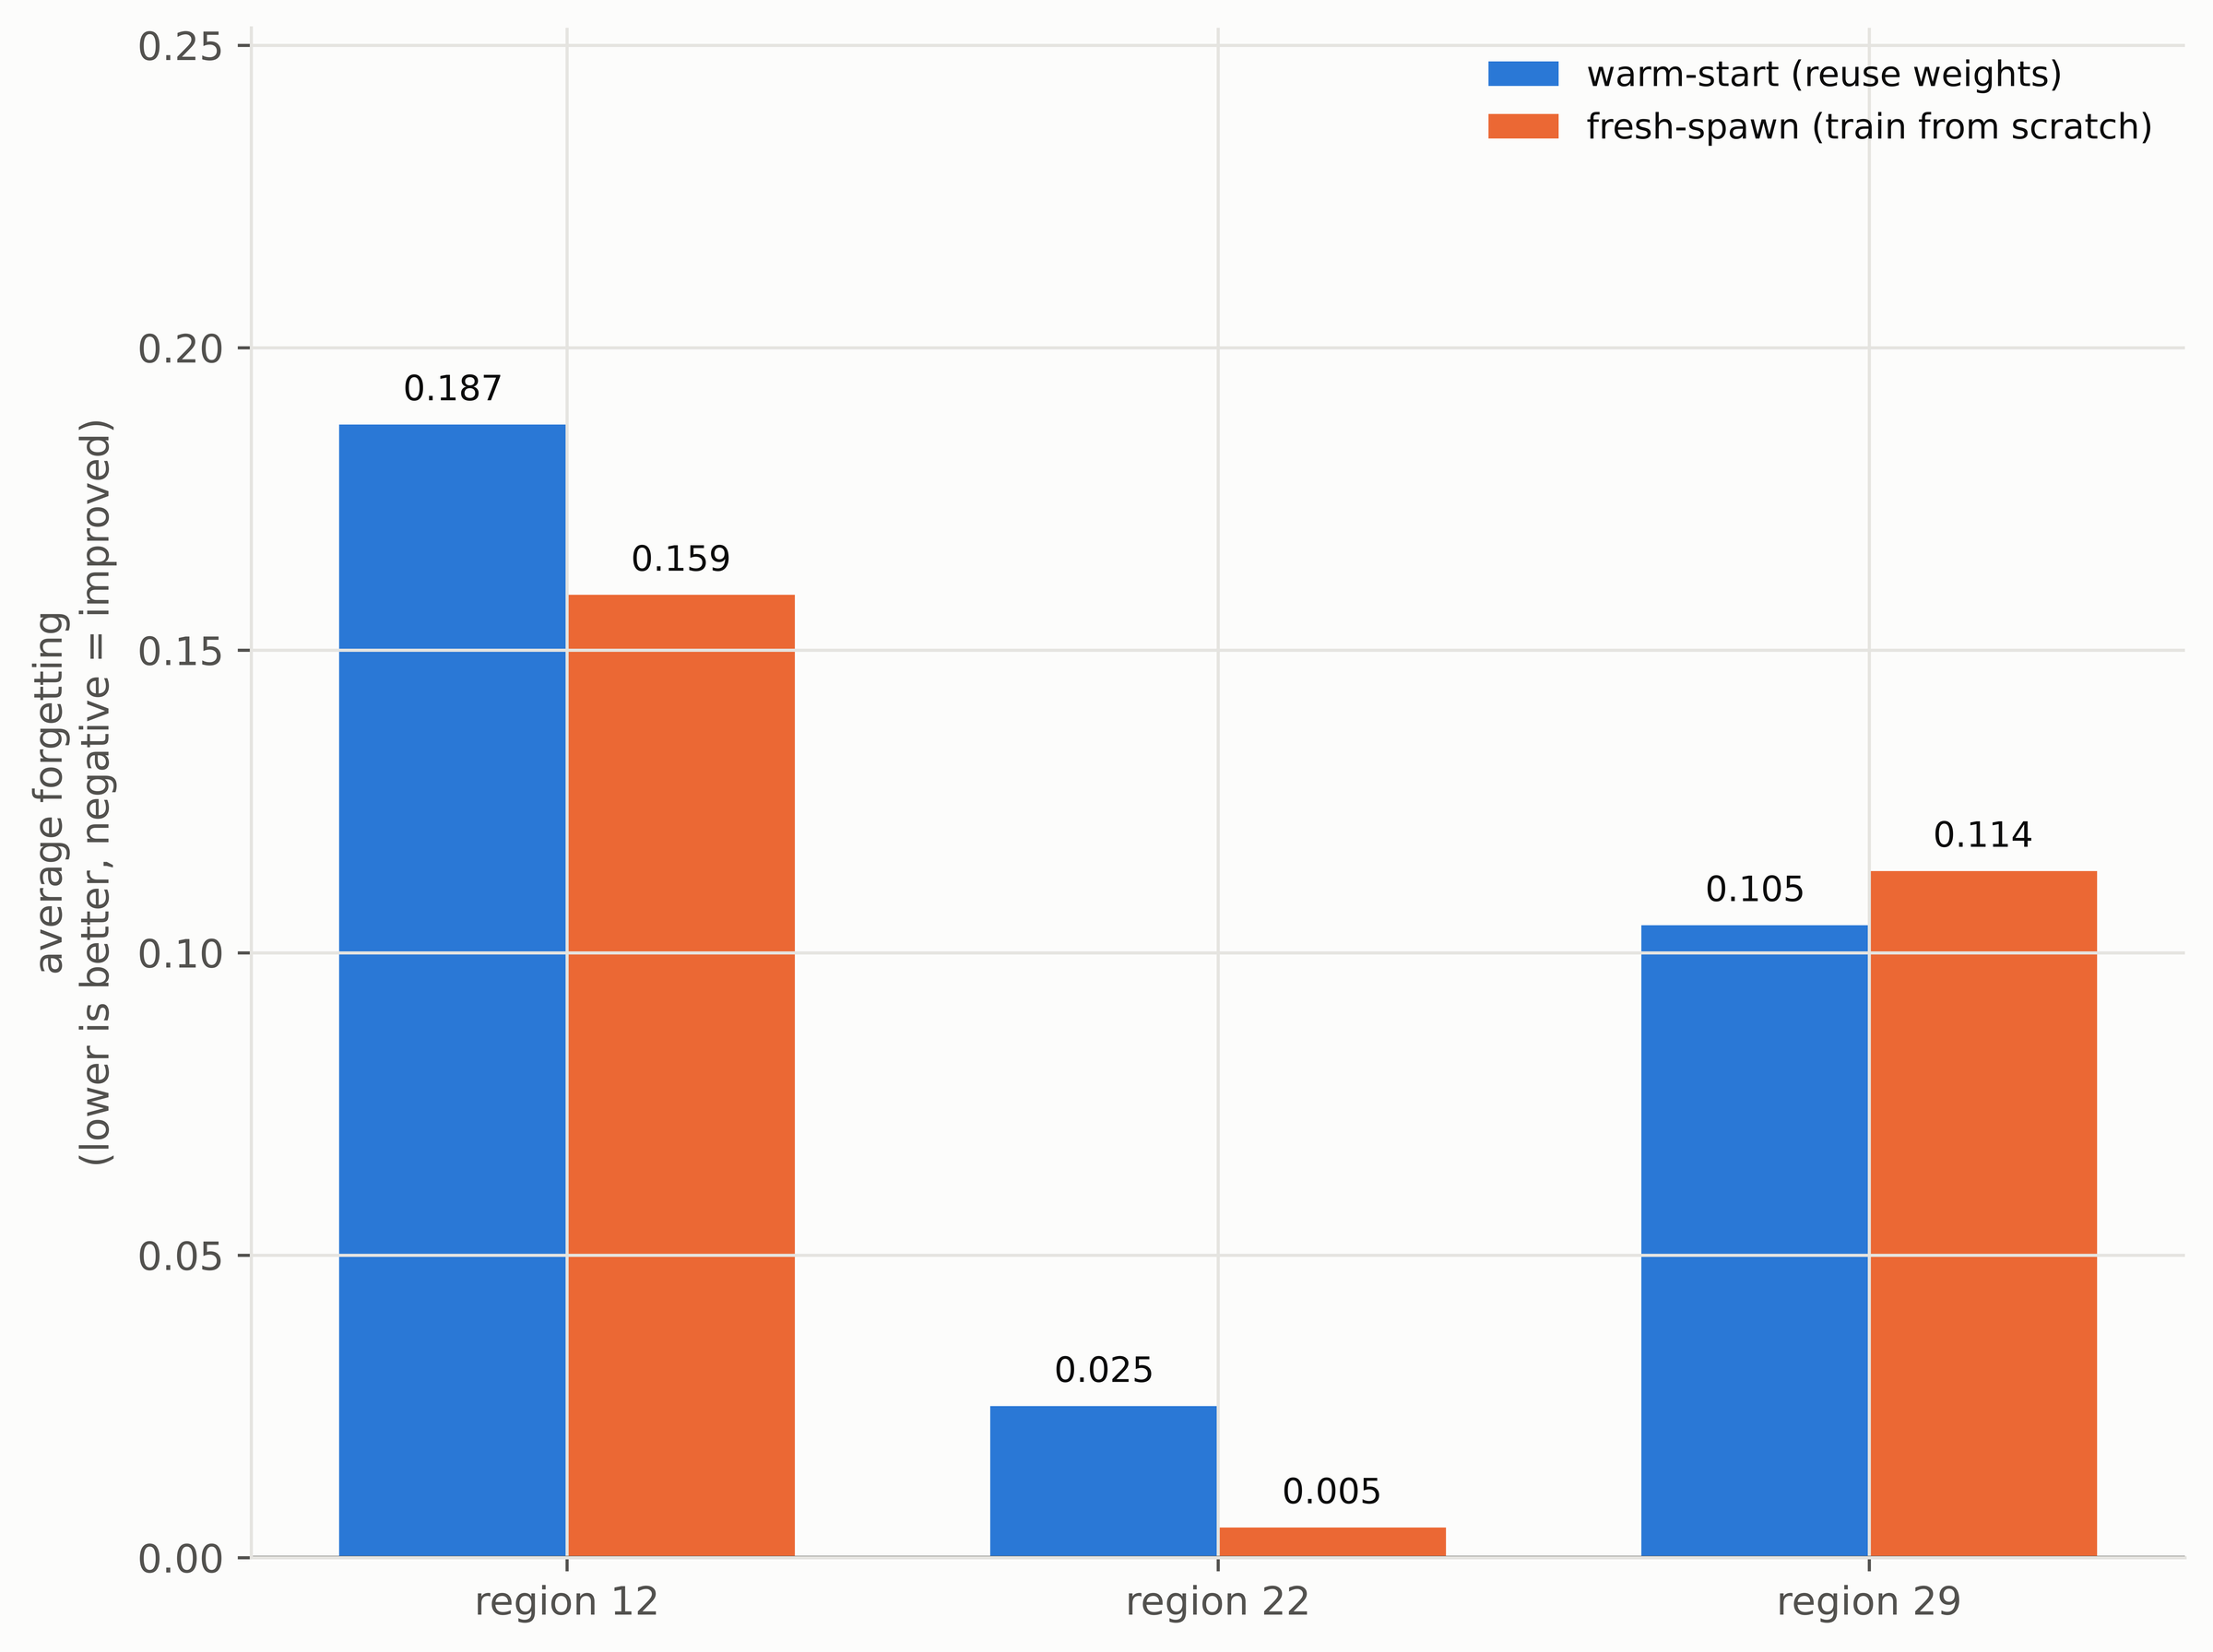
\includegraphics[width=0.62\textwidth]{ppt_forgetting_warm_vs_fresh_3regions_fixed.png}
\caption{Average forgetting (lower is better) when a reactivated expert is warm-started from its archived weights or trained fresh.}
\label{fig:forget}
\end{figure}

\section{Stage D: Structural Drift of the PCMCI Graph}
\label{sec:res-staged}

A Ni\~{n}o-3.4 proxy computed from the project's own SST matches the known ENSO phase in 22 of 24 labelled years. With one-season windows, the parent-set distance is 0.164 when the ENSO phase changes and 0.151 when it does not (Mann--Whitney $p=0.20$); with three-season windows it is 0.200 versus 0.207 ($p=0.76$). Each window has only one or two parents per target, so set membership changes mainly through sampling noise (Figure~\ref{fig:staged}).

\begin{figure}[htbp]
\centering
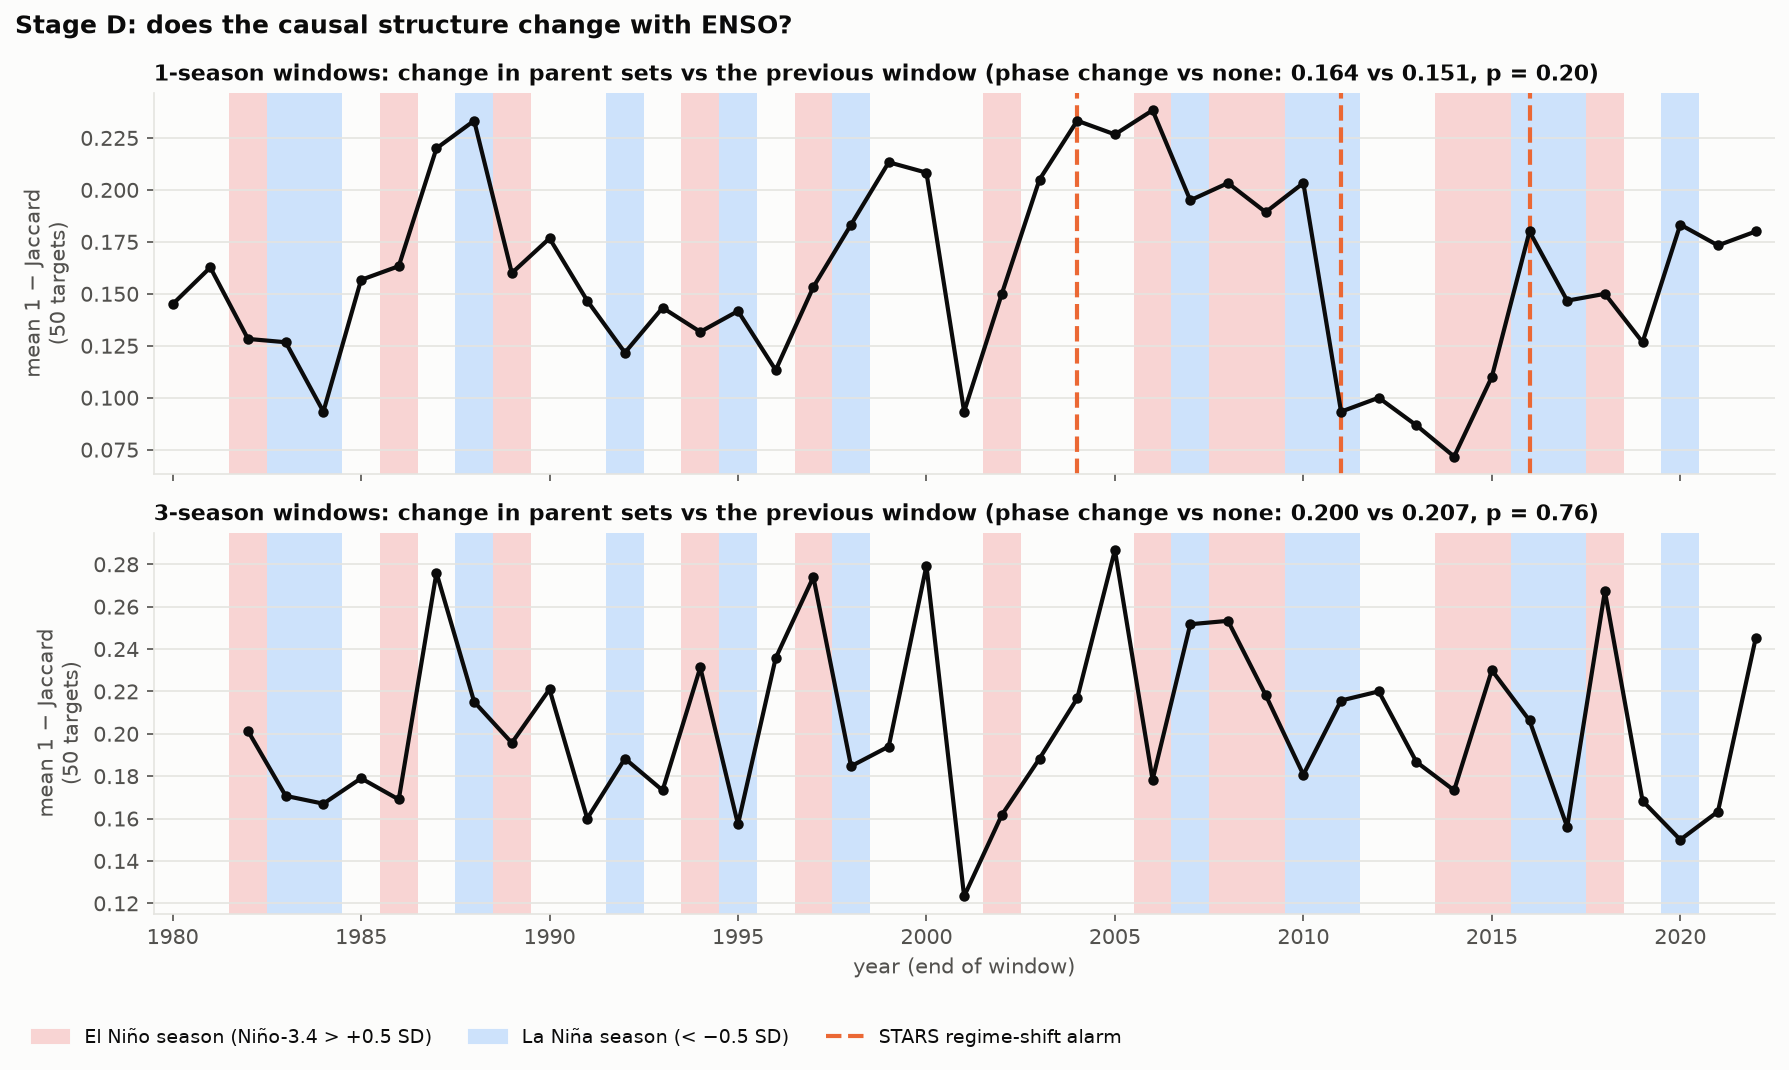
\includegraphics[width=\textwidth]{08_stage_d_drift.png}
\caption{Stage~D: mean parent-set distance between consecutive one-season (top) and three-season (bottom) windows, with El Ni\~{n}o (red) and La Ni\~{n}a (blue) seasons shaded and STARS alarms dashed.}
\label{fig:staged}
\end{figure} Unlike the splitter-score signal of Section~\ref{sec:res-drift}, the discrete PCMCI parent set is therefore not a reliable regime signal at these window lengths; longer windows and strength-based distances are the natural next step.

\section{Summary of Findings}
\label{sec:res-interpret}

\begin{table}[htbp]
\centering
\caption{Outcome of the hypotheses.}
\label{tab:hyp-outcome}
\footnotesize
\renewcommand{\arraystretch}{1.2}
\begin{tabularx}{\textwidth}{>{\raggedright\arraybackslash}p{3.6cm}>{\raggedright\arraybackslash}X>{\raggedright\arraybackslash}p{2.6cm}}
\toprule
\textbf{Hypothesis} & \textbf{Evidence} & \textbf{Outcome} \\
\midrule
H1 Credibility & 0/250 decoys; 3/536 speed violations & Supported \\
H2 Resolution persistence & 33/48 targets $\ge$ 0.5; mean 0.62 & Supported \\
H3 Graph prior helps & Informative splitters 0 $\to$ 24 (7 d) and 0 $\to$ 36 (1 d); 1-day skill better in 32/50 regions; 7-day skill unchanged & Supported at 1 day \\
H4 Earlier detection & Structure channel 2.4--9.9$\times$ faster at regions 22 and 29 & Supported at 2 of 3 regions \\
H5 Regime reuse & 104/171 changes reactivated an archived expert; blend best & Supported \\
\bottomrule
\end{tabularx}
\end{table}

\section{Limitations}
\label{sec:res-validity}

\begin{itemize}
  \item \textbf{No ground truth.} The checks can reject a bad graph but cannot prove a graph correct; every causal claim is a statement of conditional dependence between region means.
  \item \textbf{Hidden drivers and power.} PCMCI assumes all common drivers are observed; BSISO phase, ENSO and moisture are only partly captured. With 18{,}000 candidates per target, some links are missed and some false links remain.
  \item \textbf{Time-scale match.} The validated links act within one or two days, shorter than the 7-day lead; a graph built with lags of at least seven days is needed for week-ahead guidance.
  \item \textbf{Evaluation scope.} The forecasting comparisons use a single training seed and compare against the no-prior model; the drift and lifecycle results cover three regions. The upstream climatology (1979--2014) overlaps the test period by two years.
  \item \textbf{Absolute skill at 7 days.} At seven days the models beat persistence everywhere but not climatology on average ($R^2_{\mathrm{clim}}\approx-0.015$).
\end{itemize}

\section{Implications for Phase 2}
\label{sec:res-implications}

Phase~2 keeps the validation pipeline (decoys, speed mask, persistence), the activity-based season and the region-level prior; builds graphs with lags matched to the forecast lead; uses the dual-channel detector with continuous structure signals; and adopts pooled reactivation of archived experts as the default lifecycle action.
